% =====================================================================
%  Unit 2 -- Hybrid models
%  (this file is assembled from src/ch02/*.tex by build_chapter.py)
% =====================================================================
\chapter{Hybrid Models}\label{ch:hybrid}

In September 2009, after three years of competition, Netflix\index{Netflix Prize} awarded its prize of one million dollars to a team
whose final predictions blended those of hundreds of models, combined by yet another model; combining had been the
key to every stage of the competition. And yet Netflix never put the winning blend into production: its engineers
explained that the additional accuracy\index{accuracy} did not justify the engineering effort it would have required, although they
did adopt two of the individual methods found in an earlier stage of the competition \citep{amatriain2012netflix}.
The story contains both the promise of this unit and its price.

Every learning algorithm makes assumptions, and every model makes mistakes. Instead of
searching for the single best model, we can build several and combine them. This simple
idea, often summarised as the \emph{wisdom of crowds\index{wisdom of crowds|textbf}}, is behind some of the most successful
methods of machine learning: random forests\index{random forest} and gradient boosting\index{gradient boosting}\index{boosting} dominate tabular data,
and combinations of models win most data science competitions. This unit studies how to
combine models: why combinations work, how to obtain models that are worth combining, how
to fuse their predictions, how to combine models built with different techniques, and how
to build models that know when \emph{not} to predict. We close with the price to pay:
combinations of models are harder to understand, more expensive to run, and need all the
attributes of every example.

\begin{objectives}
After studying this unit you should be able to:
\begin{itemize}
  \item explain the theoretical background that supports the combination of models
        (Condorcet\index{Condorcet's jury theorem}'s theorem, the ambiguity decomposition\index{ambiguity decomposition}, the reasons why ensembles\index{ensemble} work);
  \item distinguish the mechanisms for generating diverse models, and measure diversity\index{diversity};
  \item describe and apply the main fusion\index{fusion of models} methods (linear and product combiners\index{product combiner}, voting\index{voting},
        Bayesian model averaging\index{Bayesian model averaging}, metalearning\index{metalearning});
  \item explain and use bagging\index{bagging}, boosting, randomisation\index{randomisation}, random forests and gradient
        boosting, and know when each is preferable;
  \item combine models built with different techniques (voting, stacking\index{stacking}, cascading\index{cascading},
        mixtures of experts\index{mixture of experts});
  \item decide when a model should abstain\index{abstention} or delegate\index{delegation}: derive optimal reject rules from costs,
        evaluate cautious classifiers\index{cautious classifier}, and design delegating classifiers and cascades;
  \item know the main drawbacks of ensembles and the techniques to mitigate them, such as
        pruning and mimetic\index{mimetic classifier} models.
\end{itemize}
\end{objectives}

% ---------------------------------------------------------------------
\section{The wisdom of crowds}\label{sec:crowds}

In 1906 the statistician Francis Galton visited a livestock fair where visitors could pay a
small fee to guess the weight of an ox once slaughtered and dressed. Galton obtained the list
of estimates, and found that the middle value of the distribution, the \emph{median}, was
within one per cent of the true weight \citep{galton1907vox}: the ``vox populi'' was far
more accurate than most individual guesses. The
mean of the estimates, computed later from the same data, was even closer. The phenomenon was
popularised a century later as the \emph{wisdom of crowds\index{wisdom of crowds|textbf}} \citep{surowiecki2004wisdom}.
Crowds are wise only under certain conditions: their members must hold diverse opinions,
form them independently, and there must be a good way of aggregating them.

The same principle underlies ensemble learning. Every model has limitations and makes errors;
the aim of combining models is to manage their strengths and weaknesses so that the errors of
some are compensated by the others. Theoretical and empirical results have shown that a
combination can significantly exceed the performance of its best member.

\subsection{Condorcet's jury theorem}

The oldest formal argument in favour of combining opinions is due to the Marquis de Condorcet\index{Condorcet's jury theorem}
(1785). Suppose that $T$ voters (with $T$ odd) decide between two options by majority, that each
voter is right with probability $p$, and that they vote \emph{independently}. The number of
correct votes is then binomial, and the majority is right with probability
\begin{equation}\label{eq:condorcet}
  P_{\text{maj}}(T,p)=\sum_{k=(T+1)/2}^{T}\binom{T}{k}p^k(1-p)^{T-k}.
\end{equation}
If $p>1/2$, $P_{\text{maj}}$ grows with $T$ and tends to 1; if $p<1/2$, it decreases and tends to 0
(\cref{lst:condorcet}). A crowd of independent, better-than-random voters is almost
infallible; a crowd of worse-than-random voters is reliably wrong.

\begin{pylisting}[label={lst:condorcet}]{Accuracy of the majority vote of T independent voters}
from scipy.stats import binom

def majority_accuracy(T, p):
    """P(more than half of T independent voters are right), for odd T."""
    return binom.sf(T // 2, T, p)

sizes = (1, 5, 11, 51, 101)
for p in (0.45, 0.6, 0.7):
    accs = [f"T={T}: {majority_accuracy(T, p):.3f}" for T in sizes]
    print(f"p={p:.2f}  " + "  ".join(accs))
\end{pylisting}
\begin{pyoutput}
p=0.45  T=1: 0.450  T=5: 0.407  T=11: 0.367  T=51: 0.236  T=101: 0.156
p=0.60  T=1: 0.600  T=5: 0.683  T=11: 0.753  T=51: 0.926  T=101: 0.979
p=0.70  T=1: 0.700  T=5: 0.837  T=11: 0.922  T=51: 0.999  T=101: 1.000
\end{pyoutput}

The key assumption is independence. If the voters make correlated mistakes the benefit
shrinks. In a simple model in which, with probability $\rho$, all the voters copy a common
opinion (right with probability $p$) and otherwise vote independently, the majority is right
with probability $\rho\,p+(1-\rho)\,P_{\text{maj}}(T,p)$. With $\rho=0.3$ and $p=0.6$ the accuracy
can never exceed $0.3\cdot0.6+0.7=0.88$, however large the crowd (\cref{fig:condorcet}).

\begin{figure}[htbp]
\centering
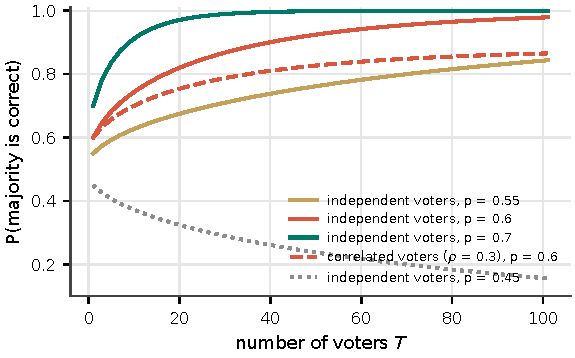
\includegraphics[width=0.74\textwidth]{ch02/condorcet}
\caption{Accuracy of a majority vote as a function of the number of voters. Independent voters
with $p>1/2$ approach perfect accuracy; correlated voters saturate; voters worse than random
($p=0.45$) get worse as the crowd grows.}
\label{fig:condorcet}
\end{figure}

For classifiers the lesson is direct. Given three models $\{h_1,h_2,h_3\}$ and a new example
$x$: if the classifiers are \emph{similar} and $h_1(x)$ is wrong, then $h_2(x)$ and $h_3(x)$ are
probably wrong too, and combining them is useless. If they are \emph{diverse}, when $h_1(x)$ is
wrong $h_2(x)$ and $h_3(x)$ may be correct, and so is the combined prediction. Combining
requires members that are both \emph{accurate} (better than random) and \emph{diverse}.

\subsection{Why do combinations work?}

\citet{dietterich2000ensemble} identified three reasons why an ensemble can be better than any of
its members:
\begin{itemize}
  \item \emph{statistical}: with limited data, many hypotheses fit the training set\index{training set} equally
        well; averaging them reduces the risk of choosing a bad one (this is the variance
        reduction of \cref{sec:biasvariance});
  \item \emph{computational}: learning algorithms perform local searches (greedy\index{multi-armed bandit!epsilon-greedy@$\varepsilon$-greedy} splits, gradient
        descent) that can get stuck in local optima; starting from different points and
        combining the results gives a better approximation;
  \item \emph{representational}: the true function may not be representable by any hypothesis of
        the class $H$, but a combination of hypotheses of $H$ may lie outside $H$ and approximate
        it better. Combining \emph{increases the expressive power} of the hypothesis language.
\end{itemize}
\Cref{fig:boundaries} illustrates the representational argument. A decision stump\index{decision stump} can only
draw one axis-parallel line (test accuracy 0.794 on the two-moons problem), but a weighted vote
of 100 stumps built by AdaBoost\index{AdaBoost} draws a complex frontier (0.902), better than a single unpruned
tree (0.855). Bagging\index{bagging}, random forests and gradient boosting\index{gradient boosting} smooth the jagged frontier of a
single tree.

\begin{figure}[htbp]
\centering
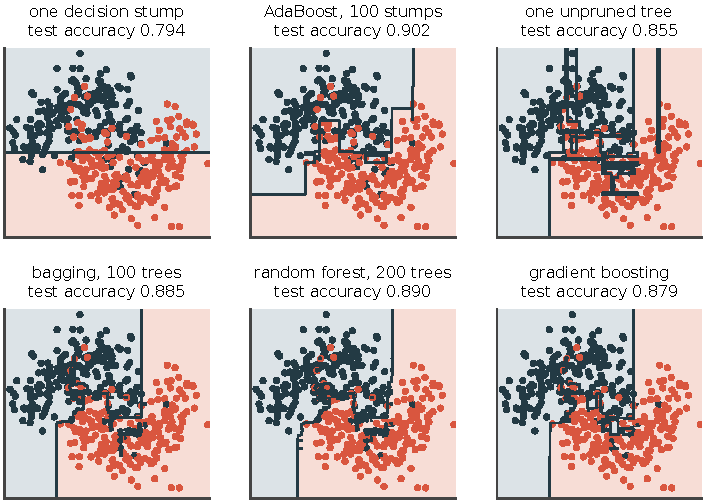
\includegraphics[width=\textwidth]{ch02/boundaries}
\caption{Decision regions on the two-moons problem (400 training examples; accuracy measured on
4000 test examples). Combinations of simple models can represent frontiers that none of their
members can.}
\label{fig:boundaries}
\end{figure}

\subsection{Diversity}

For regression with squared loss, the role of diversity\index{diversity} can be made exact. Let the ensemble
average $T$ models, $\bar f(x)=\frac1T\sum_t f_t(x)$. \citet{krogh1995neural} showed that, for any
input $x$ with target $y$,
\begin{equation}\label{eq:ambiguity}
  \underbrace{\bigl(\bar f(x)-y\bigr)^2}_{\text{ensemble error } E}
  =\underbrace{\frac1T\sum_{t=1}^{T}\bigl(f_t(x)-y\bigr)^2}_{\text{average error } \bar E}
  -\underbrace{\frac1T\sum_{t=1}^{T}\bigl(f_t(x)-\bar f(x)\bigr)^2}_{\text{ambiguity } \bar A},
\end{equation}
which follows from expanding $(f_t-y)^2=\bigl((f_t-\bar f)+(\bar f-y)\bigr)^2$ and noticing that
the deviations $f_t-\bar f$ add up to zero. The \emph{ambiguity\index{ambiguity decomposition|textbf}} $\bar A$ measures how much the
members disagree, and it is never negative: the ensemble is \emph{always} at least as good as
the average member, and it is better the more diverse the members are, provided that their
individual errors do not grow. \Cref{lst:ambiguity} checks the identity numerically for ten
bagged regression trees.

\begin{pylisting}[label={lst:ambiguity}]{The ambiguity decomposition of a bagged ensemble of regression trees}
import numpy as np
from sklearn.tree import DecisionTreeRegressor

rng = np.random.default_rng(0)
f = lambda x: np.sin(2 * np.pi * x)
X = rng.uniform(0, 1, (400, 1));     y = f(X[:, 0]) + rng.normal(0, 0.3, 400)
X_te = rng.uniform(0, 1, (2000, 1)); y_te = f(X_te[:, 0]) + rng.normal(0, 0.3, 2000)

F = []
for t in range(10):                                    # 10 trees on bootstrap samples
    i = rng.integers(0, len(y), len(y))
    F.append(DecisionTreeRegressor(max_depth=6).fit(X[i], y[i]).predict(X_te))
F = np.array(F)
f_bar = F.mean(axis=0)                                 # the ensemble prediction

E = np.mean((f_bar - y_te) ** 2)                       # error of the ensemble
E_bar = np.mean((F - y_te) ** 2)                       # average error of the members
A_bar = np.mean((F - f_bar) ** 2)                      # average ambiguity (diversity)
print(f"ensemble error        E     = {E:.4f}")
print(f"average member error  E_bar = {E_bar:.4f}")
print(f"average ambiguity     A_bar = {A_bar:.4f}")
print(f"E_bar - A_bar               = {E_bar - A_bar:.4f}")
\end{pylisting}
\begin{pyoutput}
ensemble error        E     = 0.1021
average member error  E_bar = 0.1267
average ambiguity     A_bar = 0.0247
E_bar - A_bar               = 0.1021
\end{pyoutput}

For classifiers there is no such clean decomposition, and diversity is measured with pairwise
statistics computed from the \emph{oracle outputs} of the members (correct or incorrect on each
test example) \citep{kuncheva2003measures}. For two classifiers, let $N^{11}$ be the number of
examples on which both are right, $N^{00}$ both wrong, and $N^{10}$, $N^{01}$ only one right. The
\emph{disagreement\index{diversity!disagreement|textbf}} measure and the \emph{$Q$ statistic} are
\begin{equation}
  \mathrm{dis}=\frac{N^{01}+N^{10}}{N},\qquad
  Q=\frac{N^{11}N^{00}-N^{01}N^{10}}{N^{11}N^{00}+N^{01}N^{10}},
\end{equation}
where $Q$ ranges from $-1$ to $1$ and is 0 for statistically independent classifiers. Cohen's
kappa\index{Cohen's kappa} between the predictions of two members (\cref{sec:crisp}) is another common choice. These
statistics are averaged over all pairs of members.

\begin{pylisting}[label={lst:diversity}]{Diversity and accuracy of three tree ensembles}
import numpy as np
from sklearn.datasets import make_classification
from sklearn.ensemble import (BaggingClassifier, ExtraTreesClassifier,
                              RandomForestClassifier)
from sklearn.model_selection import train_test_split
from sklearn.tree import DecisionTreeClassifier

def member_predictions(ens, X):
    feats = getattr(ens, "estimators_features_", [slice(None)] * len(ens.estimators_))
    return np.array([e.predict(X[:, f]) for e, f in zip(ens.estimators_, feats)])

def pairwise_diversity(pred, y):
    """Average disagreement and Q statistic over all pairs of members."""
    ok = pred == y                                  # correct / incorrect outputs
    dis, Q = [], []
    for i in range(len(ok)):
        for j in range(i + 1, len(ok)):
            n11, n00 = np.sum(ok[i] & ok[j]), np.sum(~ok[i] & ~ok[j])
            n10, n01 = np.sum(ok[i] & ~ok[j]), np.sum(~ok[i] & ok[j])
            dis.append((n01 + n10) / len(y))
            Q.append((n11 * n00 - n01 * n10) / (n11 * n00 + n01 * n10))
    return np.mean(dis), np.mean(Q)

X, y = make_classification(n_samples=3000, n_features=20, n_informative=10, n_redundant=4,
                           flip_y=0.05, random_state=1)
X_tr, X_te, y_tr, y_te = train_test_split(X, y, test_size=0.5, random_state=0)
ensembles = {"bagging": BaggingClassifier(DecisionTreeClassifier(), n_estimators=50,
                                          random_state=0),
             "random forest": RandomForestClassifier(50, random_state=0),
             "extra trees": ExtraTreesClassifier(50, random_state=0)}
for name, ens in ensembles.items():
    pred = member_predictions(ens.fit(X_tr, y_tr), X_te)
    dis, Q = pairwise_diversity(pred, y_te)
    print(f"{name:13s} member acc={np.mean(pred == y_te):.3f}  disagreement={dis:.3f}  "
          f"Q={Q:.3f}  ensemble acc={ens.score(X_te, y_te):.3f}")
\end{pylisting}
\begin{pyoutput}
bagging       member acc=0.803  disagreement=0.221  Q=0.659  ensemble acc=0.891
random forest member acc=0.786  disagreement=0.269  Q=0.483  ensemble acc=0.907
extra trees   member acc=0.775  disagreement=0.293  Q=0.391  ensemble acc=0.920
\end{pyoutput}

\Cref{lst:diversity} shows the typical trade-off: the members of a random forest are less
accurate than the bagged trees (0.786 against 0.803) but more diverse ($Q=0.48$ against 0.66),
and the forest is more accurate (0.907 against 0.891); extremely randomised trees\index{extra trees} push the
trade-off further. A \emph{kappa--error\index{kappa--error diagram|textbf} diagram} \citep{margineantu1997pruning} plots every pair
of members as a point (agreement, average error), and shows at a glance how each method
balances the two (\cref{fig:kappaerror}).

\begin{figure}[htbp]
\centering
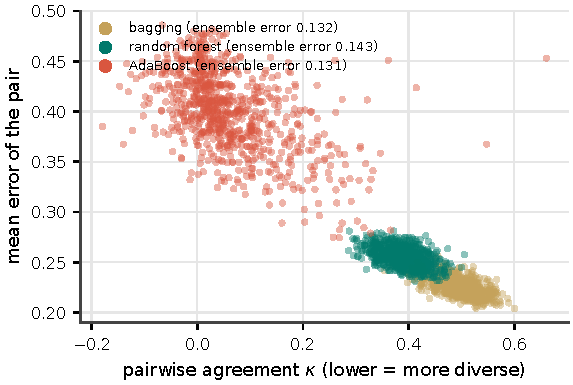
\includegraphics[width=0.74\textwidth]{ch02/kappa_error}
\caption{Kappa--error diagram of three ensembles of 40 trees. Each point is a pair of members.
Bagging produces accurate but similar members; AdaBoost produces weak but very diverse ones.}
\label{fig:kappaerror}
\end{figure}

% ---------------------------------------------------------------------
\section{Combining models}\label{sec:combining}

A combination of models has two ingredients: a way of generating a set of \emph{diverse}
models, and a way of \emph{fusing} their predictions.

\subsection{Generating diverse models}

Diverse models can be obtained by combining \emph{different learning techniques} (a neural
network, a decision tree\index{decision tree} and a nearest-neighbour\index{k-nearest neighbours@$k$-nearest neighbours} classifier), which leads to the \emph{hybrid}
methods of \cref{sec:hybrid}, or by running \emph{one learning technique} several times with
some variation, which leads to the \emph{ensemble\index{ensemble|textbf}} methods of \cref{sec:ensembles}. In the
second case, diversity\index{diversity} can be induced by:
\begin{itemize}
  \item \emph{manipulating the training examples}: each model sees a different subset or a
        different weighting of the examples (bagging\index{bagging}, boosting);
  \item \emph{manipulating the input features}: each model sees a different subset of the
        attributes, as in the random subspace method \citep{ho1998random};
  \item \emph{manipulating the classes}: the classes of the training set are modified, for
        instance by grouping them into different binary problems whose combination recovers
        the original classes, as in error-correcting output codes \citep{dietterich1995solving};
  \item \emph{injecting randomness} into the learning process: random initial weights of
        a neural network, random choices among the best splits of a tree (randomisation\index{randomisation}),
        random thresholds\index{threshold} (extremely randomised trees\index{extra trees}, \citealp{geurts2006extremely}).
\end{itemize}
\citet{brown2005diversity} distinguish \emph{implicit} diversity generation, which uses
indirect means and hopes that diversity appears (random samples, random features), from
\emph{explicit} diversity generation, which constructs each new member so that it is
substantially different from the previous ones (boosting reweights the examples the
ensemble gets wrong; Decorate\index{Decorate} adds examples that contradict it).

\subsection{Fusion methods}

Let $f_t(y\mid x)$ be the probability (or score) that model $t$ assigns to class $y$, for
$t=1,\dots,T$. The main ways of combining them are the following.

\paragraph{Linear combiner} A weighted average of the outputs,
\begin{equation}\label{eq:linear}
  \bar f(y\mid x)=\sum_{t=1}^{T}w_t\,f_t(y\mid x),
\end{equation}
applicable to regression and to soft (probabilistic) classification. With $w_t=1/T$ it is the
simple uniform average. Estimating the weights without overfitting\index{overfitting} is difficult, and in
practice the uniformly weighted average is used very often, and is hard to beat.

\paragraph{Product combiner} A (weighted) product of the probabilities,
\begin{equation}\label{eq:product}
  \bar f(y\mid x)=\frac1Z\prod_{t=1}^{T}f_t(y\mid x)^{w_t},
\end{equation}
where $Z$ is a normalisation factor that makes $\bar f$ a valid probability distribution. With non-negative
weights summing to one it is a weighted \emph{geometric mean} (a logarithmic pool); with unit exponents, as in
\cref{lst:fusion}, it is a plain normalised product, which gives sharper probabilities. If the models
use \emph{different} evidence, conditionally independent given the class, Bayes' rule gives
$P(y\mid x_1,\dots,x_T)\propto P(y)^{1-T}\prod_tP(y\mid x_t)$: multiplying posteriors counts the prior $T$ times
unless it is corrected, and calibration\index{calibration} of the members alone does not make the product optimal. The
product also has a \emph{veto} effect: a
single model that assigns a probability close to zero to a class practically eliminates it.
Again, the weights are difficult to determine. Both combiners are special cases of the
\emph{generalised mean},
\begin{equation}
  \bar f(y\mid x)=\frac1Z\Bigl(\sum_{t=1}^{T}w_t\,f_t(y\mid x)^{\alpha}\Bigr)^{1/\alpha},
\end{equation}
which, for weights summing to one, gives the linear combiner\index{linear combiner} for $\alpha=1$, the weighted geometric mean as
$\alpha\to0$, the
maximum as $\alpha\to\infty$ and the minimum as $\alpha\to-\infty$: a continuum of possible
combining strategies.

\paragraph{Voting} Each classifier votes for a class, and the class with the most votes is
selected: the \emph{majority} vote if it needs more than half of the votes, the
\emph{plurality} vote otherwise. Ties can be broken in favour of the majority class. Voting\index{voting}
works with crisp classifiers and ignores the confidence of the members. \emph{Weighted} voting
gives each member a weight, again difficult to establish.

\begin{example}{Three ways of fusing three models}{fusion}
Three models assign these probabilities to the classes A and B for an example:
$h_1=(0.90,0.10)$, $h_2=(0.45,0.55)$ and $h_3=(0.40,0.60)$. Two of the three models prefer B,
so the majority vote predicts B. The average is $(0.583,0.417)$, which predicts A: the
confident opinion of $h_1$ outweighs the two lukewarm votes for B. The normalised product is
$(0.831,0.169)$, which also predicts A (\cref{lst:fusion}). Voting counts heads; averaging
weighs confidence.
\end{example}

\begin{pylisting}[label={lst:fusion}]{Majority vote, linear combiner and product combiner}
import numpy as np

# Probabilities of the classes (A, B) given by three models to one example
P = np.array([[0.90, 0.10],
              [0.45, 0.55],
              [0.40, 0.60]])
classes = np.array(["A", "B"])

votes = np.bincount(P.argmax(axis=1), minlength=2)   # majority voting
mean = P.mean(axis=0)                                 # linear combiner (uniform)
prod = P.prod(axis=0) / P.prod(axis=0).sum()          # product combiner (normalised)
print("votes:  ", votes, "->", classes[votes.argmax()])
print("mean:   ", mean.round(3), "->", classes[mean.argmax()])
print("product:", prod.round(3), "->", classes[prod.argmax()])
\end{pylisting}
\begin{pyoutput}
votes:   [1 2] -> B
mean:    [0.583 0.417] -> A
product: [0.831 0.169] -> A
\end{pyoutput}

\paragraph{Bayesian model averaging} From a Bayesian perspective, using only one model ignores
the uncertainty of having a partial view of the problem, represented by the training data $D$.
Bayesian model averaging\index{Bayesian model averaging} (BMA) combines all the models $h$ of the hypothesis space, weighted by
their posterior probability \citep{hoeting1999bayesian}:
\begin{equation}
  P(y\mid x,D)=\sum_{h}P(y\mid x,h)\,P(h\mid D),
  \qquad
  P(h\mid D)\propto P(D\mid h)\,P(h),
\end{equation}
where $P(h)$ is the prior probability of model $h$ and $P(D\mid h)$ its likelihood. BMA propagates
the uncertainty over the candidate models; it is coherent when the model space, the priors and the
likelihood are adequate, and its behaviour depends on all of them and on the prediction objective. When
every candidate is misspecified, the posterior may concentrate on a single model as data grow, so BMA
behaves more like model \emph{selection} than like an ensemble, even when a mixture would predict better
\citep{domingos2000bayesian,yao2018using}. Cross-validated stacking\index{stacking} (\cref{sec:hybrid}) instead chooses
the weights to optimise predictive performance: the two methods answer different questions.

\paragraph{Metalearning} Instead of fixing the fusion\index{fusion of models} rule, we can \emph{learn} it: a second-level
model is trained to combine the predictions of the members. This requires extra (validation)
data, since the combiner must be trained on predictions made on examples that the members have
not seen. Stacking and cascading\index{cascading} (\cref{sec:hybrid}) are the main examples.

% ---------------------------------------------------------------------
\section{Ensemble methods}\label{sec:ensembles}

Ensemble methods generate many models with a single learning technique, most often decision
trees, and combine them. \Cref{fig:bagboost} contrasts the two classic families: bagging\index{bagging} builds
its members independently and in parallel; boosting builds them sequentially, each one focused
on the mistakes of the previous ones.

\begin{figure}[htbp]
\centering
\begin{tikzpicture}[font=\scriptsize\sffamily,
  box/.style={draw=edmnavy,fill=edmnavy!6,rounded corners=2pt,minimum width=15mm,minimum height=6mm,align=center},
  mod/.style={draw=edmteal,fill=edmteal!10,rounded corners=2pt,minimum width=13mm,minimum height=6mm,align=center},
  fus/.style={draw=edmcoral,fill=edmcoral!10,rounded corners=2pt,minimum width=14mm,minimum height=7mm,align=center},
  arr/.style={-{Stealth[length=1.8mm]},edmnavy}]
  % ---- bagging
  \node[box] (d) at (0,0) {training\\data};
  \foreach \i/\y in {1/1.1,2/0,3/-1.1}{
    \node[box,minimum width=17mm] (b\i) at (2.3,\y) {bootstrap\\sample \i};
    \node[mod] (m\i) at (4.4,\y) {model \i};
    \draw[arr] (d.east) -- (b\i.west);
    \draw[arr] (b\i) -- (m\i);
  }
  \node[fus] (v) at (6.3,0) {uniform\\vote};
  \foreach \i in {1,2,3} \draw[arr] (m\i.east) -- (v.west);
  \node[font=\small\sffamily\bfseries,text=edmnavy] at (3.2,1.9) {Bagging};
  % ---- boosting
  \begin{scope}[xshift=7.6cm]
    \foreach \i/\y in {1/1.1,2/0,3/-1.1}{
      \node[box,minimum width=17mm] (w\i) at (0.9,\y) {weighted\\data, round \i};
      \node[mod] (n\i) at (3.0,\y) {model \i\\[-1pt]$\alpha_\i$};
      \draw[arr] (w\i) -- (n\i);
    }
    \draw[arr,edmcoral] (n1.south west) -- node[left,pos=0.3,text=edmcoral] {reweight} (w2.north east);
    \draw[arr,edmcoral] (n2.south west) -- node[left,pos=0.3,text=edmcoral] {reweight} (w3.north east);
    \node[fus] (wv) at (4.9,0) {weighted\\vote};
    \foreach \i in {1,2,3} \draw[arr] (n\i.east) -- (wv.west);
    \node[font=\small\sffamily\bfseries,text=edmnavy] at (2.0,1.9) {Boosting};
  \end{scope}
\end{tikzpicture}
\caption{Bagging trains its members independently on bootstrap samples and combines them with a
uniform vote. Boosting trains them sequentially on reweighted data, increasing the weight of the
examples misclassified so far, and combines them with a weighted vote.}
\label{fig:bagboost}
\end{figure}

\subsection{Bagging}

\emph{Bagging\index{bagging|textbf}} (bootstrap\index{bootstrap} aggregating) was proposed by \citet{breiman1996bagging}. Each member of
the ensemble is learned from a different data set, a \emph{bootstrap sample} obtained by drawing
$n$ examples uniformly at random and with replacement from the $n$ training examples
(\cref{sec:protocols}); the members are combined with a uniform vote, or by averaging their
probabilities. The only parameter is the size $T$ of the ensemble.

Bagging is an implicit diversity\index{diversity} generation method, and it works because averaging reduces
variance. If the predictions of the members are identically distributed random variables with
variance $\sigma^2$ and pairwise correlation $\rho$, the variance of their average is
\citep[Section~15.2]{hastie2009elements}
\begin{equation}\label{eq:avgvar}
  \Var\Bigl(\frac1T\sum_{t=1}^{T}f_t(x)\Bigr)=\rho\,\sigma^2+\frac{1-\rho}{T}\,\sigma^2 .
\end{equation}
The second term vanishes as $T$ grows, but the first one does not: the benefit of bagging is
limited by the correlation between its members. Two practical consequences follow:
\begin{itemize}
  \item bagging works well with \emph{unstable} models, those that change a lot with small
        changes of the training data (unpruned trees, neural networks), and does little for
        stable ones ($k$-NN, linear models), whose bootstrap replicas are almost identical;
  \item about 36.8\% of the training examples are left out of each bootstrap sample, so every
        training example can be predicted by the members that did not see it. This
        \emph{out-of-bag\index{out-of-bag estimate|textbf}} (OOB) estimate gives an almost free estimate of the generalisation\index{generalisation}
        performance.
\end{itemize}
Since the members are independent, bagging is trivially parallelised.

\subsection{Boosting}

Boosting builds the ensemble sequentially. AdaBoost\index{AdaBoost} \citep{freund1996experiments,freund1997decision},
the most popular algorithm of the family, keeps a weight for each training example. In each
round a new model is trained with the current weights, the weights of the examples it
misclassifies are increased, and those of the correct ones decreased, so that the next model
focuses on the examples that the ensemble finds difficult. Each model also receives a weight
$\alpha_t$ that depends on its accuracy, and the final prediction is a weighted vote
(\cref{alg:adaboost}). The algorithm stops when a limit of $T$ models is reached or when a
model is no better than random.

\begin{algorithm}[htbp]
\caption{AdaBoost (binary classes $y\in\{-1,+1\}$)}\label{alg:adaboost}
\begin{algorithmic}[1]
\Require training set $\{(x_i,y_i)\}_{i=1}^{n}$; base learner; number of rounds $T$
\State $w_i\gets1/n$ for $i=1,\dots,n$
\For{$t=1,\dots,T$}
  \State train $h_t$ with weights $w$
  \State $\varepsilon_t\gets\sum_{i:\,h_t(x_i)\neq y_i}w_i$ \Comment{weighted error}
  \If{$\varepsilon_t=0$} \textbf{return} $h_t$ \Comment{perfect on the training data} \EndIf
  \If{$\varepsilon_t\geq1/2$} \textbf{stop} \Comment{no weak learner found} \EndIf
  \State $\alpha_t\gets\frac12\ln\frac{1-\varepsilon_t}{\varepsilon_t}$ \Comment{weight of the model}
  \State $w_i\gets w_i\,e^{\alpha_t}$ if $h_t(x_i)\neq y_i$, and $w_i\gets w_i\,e^{-\alpha_t}$ otherwise
  \State normalise $w$ so that $\sum_i w_i=1$
\EndFor
\State \Return $H(x)=\operatorname{sign}\bigl(\sum_{t}\alpha_t\,h_t(x)\bigr)$
\end{algorithmic}
\end{algorithm}

\begin{example}{One round of AdaBoost}{adaround}
Ten training examples start with weight 0.1 each, and the first model misclassifies three of
them, so $\varepsilon_1=0.3$ and $\alpha_1=\frac12\ln(0.7/0.3)=0.424$. The weights of the three
mistakes are multiplied by $e^{0.424}=1.528$ and those of the seven correct examples by
$e^{-0.424}=0.655$. After normalising, each mistake weighs $1/6$ and each correct example
$1/14$: the misclassified examples, 30\% of the data, now carry half of the total weight. In
fact, after every update the previous model has weighted error exactly 0.5, so the next model
is forced to learn something different: boosting generates diversity\index{diversity} \emph{explicitly}.
\end{example}

\Cref{lst:adaboost} implements \cref{alg:adaboost} in a few lines and obtains exactly the same
accuracy as scikit-learn's implementation: 100 decision stumps\index{decision stump} combine into a classifier with a test accuracy of 0.915. The first stump
reaches 0.781, but the later ones fit differently weighted versions of the training data, and on the
original test data\index{test set} their mean accuracy is only 0.557: a weak learner\index{weak learner} must be better than random on
the weighted data of its round, not on the original distribution.

\begin{pylisting}[label={lst:adaboost}]{AdaBoost written from scratch and compared with scikit-learn}
import numpy as np
from sklearn.datasets import make_classification
from sklearn.ensemble import AdaBoostClassifier
from sklearn.model_selection import train_test_split
from sklearn.tree import DecisionTreeClassifier

X, y01 = make_classification(n_samples=2000, n_features=10, n_informative=5,
                             random_state=4)
y = 2 * y01 - 1                                   # AdaBoost uses labels in {-1, +1}
X_tr, X_te, y_tr, y_te = train_test_split(X, y, test_size=0.5, random_state=0)

w = np.full(len(y_tr), 1 / len(y_tr))             # uniform initial weights
stumps, alphas = [], []
for t in range(100):
    h = DecisionTreeClassifier(max_depth=1).fit(X_tr, y_tr, sample_weight=w)
    miss = h.predict(X_tr) != y_tr
    eps = w[miss].sum()                           # weighted training error
    if eps == 0 or eps >= 0.5:                    # perfect, or no weak learner
        break
    alpha = 0.5 * np.log((1 - eps) / eps)         # weight of the new member
    w *= np.exp(np.where(miss, alpha, -alpha))    # mistakes gain weight
    w /= w.sum()
    stumps.append(h)
    alphas.append(alpha)
    if t < 3:
        print(f"round {t + 1}: weighted error={eps:.3f}  alpha={alpha:.3f}")

F = sum(a * h.predict(X_te) for a, h in zip(alphas, stumps))
print(f"our AdaBoost (100 stumps):  test accuracy={np.mean(np.sign(F) == y_te):.3f}")
ada = AdaBoostClassifier(DecisionTreeClassifier(max_depth=1), n_estimators=100,
                         random_state=0).fit(X_tr, y_tr)
print(f"scikit-learn's AdaBoost:    test accuracy={ada.score(X_te, y_te):.3f}")
print(f"the first stump:            test accuracy={stumps[0].score(X_te, y_te):.3f}")
mean_acc = np.mean([h.score(X_te, y_te) for h in stumps])
print(f"mean of the 100 stumps:      test accuracy={mean_acc:.3f}")
\end{pylisting}
\begin{pyoutput}
round 1: weighted error=0.219  alpha=0.636
round 2: weighted error=0.264  alpha=0.512
round 3: weighted error=0.281  alpha=0.470
our AdaBoost (100 stumps):  test accuracy=0.915
scikit-learn's AdaBoost:    test accuracy=0.915
the first stump:            test accuracy=0.781
mean of the 100 stumps:      test accuracy=0.557
\end{pyoutput}

AdaBoost has an elegant theory. Its training error is bounded by
$\prod_t2\sqrt{\varepsilon_t(1-\varepsilon_t)}$, which decreases exponentially with $T$ when every
member keeps a weighted error of at most $1/2-\gamma$ for a fixed $\gamma>0$ (a \emph{weak learner}): the
bound is then at most $e^{-2\gamma^2T}$. That is a statement about the training error; the good generalisation\index{generalisation}
of AdaBoost
has been explained in terms of the \emph{margins} of the training examples
\citep{schapire1998boosting}. AdaBoost can also be seen as a greedy\index{multi-armed bandit!epsilon-greedy@$\varepsilon$-greedy} minimisation of the
exponential loss $\sum_i e^{-y_iF(x_i)}$, with $F(x)=\sum_t\alpha_th_t(x)$
\citep{friedman2000additive}. This last view explains its main weakness: the exponential loss
grows very fast for examples with large negative margins, so mislabelled\index{label noise} examples receive
enormous weights. \emph{Boosting\index{boosting|textbf} is vulnerable to noisy data}, as we will see in
\cref{sec:performance}.

\subsection{Gradient boosting}

\emph{Gradient boosting\index{gradient boosting|textbf}\index{boosting|textbf}} \citep{friedman2001greedy} generalises the idea to any differentiable
loss $\ell$. The model is an additive expansion $F_T(x)=F_0(x)+\sum_{t=1}^{T}\nu\,h_t(x)$; at each
step, a new model $h_t$ (usually a small regression tree) is fitted to the \emph{negative
gradient} of the loss with respect to the current predictions,
\begin{equation}
  r_{it}=-\frac{\partial\,\ell\bigl(y_i,F(x_i)\bigr)}{\partial F(x_i)}\Big|_{F=F_{t-1}},
\end{equation}
which for the squared loss is simply the residual\index{residual analysis} $y_i-F_{t-1}(x_i)$: each new tree predicts the
errors of the previous ones, and its predictions are added to the ensemble. The \emph{learning
rate\index{learning rate|textbf}} (shrinkage) $\nu\in(0,1]$ slows down the learning, which improves generalisation\index{generalisation} at the
cost of more trees; the number of trees is usually chosen by \emph{early stopping\index{early stopping|textbf}} on a
validation set\index{validation set}.

Efficient implementations of gradient boosting with regularisation, histogram-based splits and
careful engineering, such as XGBoost\index{XGBoost} \citep{chen2016xgboost}, LightGBM \citep{ke2017lightgbm} and
CatBoost \citep{prokhorenkova2018catboost}, have dominated applied machine learning on
\emph{tabular} data and data science competitions for a decade. scikit-learn's
\code{HistGradientBoostingClassifier} follows the same design (\cref{lst:gb}).

\begin{pylisting}[label={lst:gb}]{Random forest, gradient boosting and histogram gradient boosting with early stopping}
from sklearn.datasets import make_classification
from sklearn.ensemble import (GradientBoostingClassifier, HistGradientBoostingClassifier,
                              RandomForestClassifier)
from sklearn.metrics import roc_auc_score
from sklearn.model_selection import train_test_split

X, y = make_classification(n_samples=20000, n_features=30, n_informative=12, n_redundant=6,
                           flip_y=0.05, class_sep=0.8, random_state=2)
X_tr, X_te, y_tr, y_te = train_test_split(X, y, test_size=0.5, random_state=0)
models = {
    "random forest (300 trees)": RandomForestClassifier(300, n_jobs=-1, random_state=0),
    "gradient boosting (300 trees)": GradientBoostingClassifier(n_estimators=300,
                                                                random_state=0),
    "histogram GB + early stopping": HistGradientBoostingClassifier(
        max_iter=2000, early_stopping=True, n_iter_no_change=30, random_state=0)}
for name, m in models.items():
    auc = roc_auc_score(y_te, m.fit(X_tr, y_tr).predict_proba(X_te)[:, 1])
    used = f"   (trees used: {m.n_iter_})" if hasattr(m, "n_iter_") else ""
    print(f"{name:30s} AUC={auc:.4f}{used}")
\end{pylisting}
\begin{pyoutput}
random forest (300 trees)      AUC=0.9682
gradient boosting (300 trees)  AUC=0.9631
histogram GB + early stopping  AUC=0.9687   (trees used: 224)
\end{pyoutput}

\subsection{Bagging versus boosting}

\Cref{tab:bagboost} summarises the main differences. Boosting usually obtains better accuracy
with clean data, while bagging\index{bagging} is more robust in noisy contexts and easier to parallelise.

\begin{table}[htbp]
\centering\small
\caption{Bagging and AdaBoost compared. Gradient boosting is also sequential, but it fits
pseudo-residuals, adds up the contributions of its members, and its sensitivity to noise depends on
the loss.}\label{tab:bagboost}
\begin{tabularx}{\textwidth}{@{}>{\raggedright\arraybackslash}p{3.2cm}XX@{}}
\toprule
& Bagging & AdaBoost\\
\midrule
Training data of each member & bootstrap sample & all data, reweighted (or resampled)\\
Construction & independent, parallel & sequential\\
Diversity & implicit & explicit (focus on the mistakes)\\
Fusion & unweighted (uniform) vote or average & weighted vote ($\alpha_t$)\\
Number of members & always $T$ & $T$ is a limit; may stop earlier\\
Main effect & reduces variance & reduces bias (and variance)\\
Best base models & unstable, low bias (deep trees) & weak learners (stumps, small trees)\\
Accuracy & good & usually better\\
Label noise & robust in many problems & sensitive (exponential loss)\\
\bottomrule
\end{tabularx}
\end{table}

\subsection{Randomisation}

\citet{dietterich2000experimental} proposed a very simple way of generating diverse decision
trees: \emph{randomisation\index{randomisation|textbf}} injects randomness into the internal decisions of the learning
algorithm. When choosing the split of a node, instead of always taking the best one, the
algorithm chooses uniformly at random among the 20 best splits. Each run generates a different
tree, and the trees are combined by uniform voting\index{voting}. Unlike bagging\index{bagging}, every tree is learned from
all the training data.

\subsection{Multi-trees}

Ensembles of trees store many trees that share much of their structure: many members split on
the same attribute at the root. A \emph{multi-tree\index{multi-tree|textbf}} \citep{estruch2002shared} stores all of them
in a single structure. During the induction of a decision tree, the splits that are not chosen
at a node are not discarded but stored as \emph{suspended} nodes, which turns the tree into an
AND/OR tree (\cref{fig:multitree}): OR-nodes represent alternative splits, and AND-nodes the
branches of a split. Activating different combinations of suspended OR-nodes generates
different trees, and the number of trees grows exponentially with the number of exploited
OR-nodes, while the resources needed grow only sublinearly, because the trees share their
common parts. The population is generated by selecting which suspended node to explore next
according to different criteria (optimality, depth, randomness), and the trees can be fused in
different ways, or a single tree can be extracted following the Occam principle. Multi-trees
achieve accuracies similar to bagging\index{bagging} and boosting with fewer resources (time and memory), and
they can even replicate bagging while sharing the common parts of the trees.

\begin{figure}[htbp]
\centering
\begin{tikzpicture}[font=\scriptsize\sffamily,
  ornode/.style={circle,draw=edmcoral,fill=edmcoral!15,minimum size=5mm,inner sep=0pt},
  andnode/.style={rectangle,draw=edmnavy,fill=edmnavy!8,minimum size=4.5mm,inner sep=1pt},
  leaf/.style={rectangle,rounded corners=1.5pt,draw=edmteal,fill=edmteal!10,inner sep=2pt},
  level distance=10mm]
  \node[ornode] (r) at (0,0) {OR};
  \node[andnode] (a1) at (-3,-1.1) {$X_1$};
  \node[andnode,dashed] (a2) at (3,-1.1) {$X_3$};
  \draw (r) -- (a1); \draw[dashed] (r) -- (a2);
  \node[leaf] (l1) at (-4.2,-2.2) {Yes};
  \node[ornode] (o2) at (-1.8,-2.2) {OR};
  \draw (a1) -- node[left,font=\tiny] {$\leq0.5$} (l1);
  \draw (a1) -- node[right,font=\tiny] {$>0.5$} (o2);
  \node[andnode] (a3) at (-2.7,-3.3) {$X_2$};
  \node[andnode,dashed] (a4) at (-0.9,-3.3) {$X_4$};
  \draw (o2) -- (a3); \draw[dashed] (o2) -- (a4);
  \node[leaf] (l2) at (-3.3,-4.3) {Yes};
  \node[leaf] (l3) at (-2.1,-4.3) {No};
  \draw (a3) -- (l2); \draw (a3) -- (l3);
  \node[leaf,dashed] (l4) at (-1.3,-4.3) {No};
  \node[leaf,dashed] (l5) at (-0.4,-4.3) {Yes};
  \draw[dashed] (a4) -- (l4); \draw[dashed] (a4) -- (l5);
  \node[leaf,dashed] (l6) at (2.3,-2.2) {Yes};
  \node[leaf,dashed] (l7) at (3.7,-2.2) {No};
  \draw[dashed] (a2) -- (l6); \draw[dashed] (a2) -- (l7);
  \node[align=left,anchor=west,font=\scriptsize\sffamily] at (1.2,-3.6)
    {solid: tree currently selected\\dashed: suspended alternatives};
\end{tikzpicture}
\caption{A small multi-tree. OR-nodes keep alternative splits; choosing an alternative at each OR-node that is
reached yields one of the trees of the ensemble. Choosing $X_1$ at the root gives two trees ($X_2$ or $X_4$
on its right branch) and choosing $X_3$ gives a third one: a choice in an unreached subtree does not
create a new tree. All the trees share the common parts of the structure.}
\label{fig:multitree}
\end{figure}

\subsection{Random forests}

A \emph{random forest\index{random forest|textbf}} \citep{breiman2001random} is a hybrid of bagging\index{bagging} and the random subspace
method. Each tree is learned from a bootstrap\index{bootstrap} sample, and at each node the best split is chosen
only among a random subset of $m$ of the $M$ attributes. Breiman suggested
$m=\lfloor\log_2 M+1\rfloor$; the usual recommendations are $m=\sqrt M$ for classification and
$m=M/3$ for regression (the defaults of R's \textsf{randomForest}); \textsf{scikit-learn} uses $\sqrt M$ for
classification but, by default, all the attributes for regression. The trees are grown without pruning, so each one overfits its own
bootstrap sample, and they are combined by unweighted voting\index{voting} (or by averaging their
probabilities). Restricting the candidate attributes decorrelates the trees, which reduces the
first term of \cref{eq:avgvar}: a random forest is bagging with more diversity\index{diversity}.
\emph{Extremely randomised trees\index{extra trees|textbf}} \citep{geurts2006extremely} go one step further and choose the
thresholds of the splits at random as well. \Cref{lst:bagging} compares a single tree, bagging,
random forests and extra trees: each additional source of randomness improves the ensemble, and
the OOB\index{out-of-bag estimate} estimates are close to the test accuracies.

\begin{pitfall}
\textbf{A random forest that is not one.} In \textsf{scikit-learn}, \code{RandomForestRegressor()} with its default
parameters considers every attribute at every split (\code{max\_features=1.0}): it is bagging of regression trees,
not a random forest. Set \code{max\_features}, for instance to $1/3$ or \code{"sqrt"}, to decorrelate the trees.
\end{pitfall}

\begin{pylisting}[label={lst:bagging}]{A single tree versus three bagging-type ensembles, with out-of-bag estimates}
from sklearn.datasets import make_classification
from sklearn.ensemble import (BaggingClassifier, ExtraTreesClassifier,
                              RandomForestClassifier)
from sklearn.model_selection import train_test_split
from sklearn.tree import DecisionTreeClassifier

X, y = make_classification(n_samples=3000, n_features=20, n_informative=10, n_redundant=4,
                           flip_y=0.05, random_state=1)
X_tr, X_te, y_tr, y_te = train_test_split(X, y, test_size=0.5, random_state=0)
models = {
    "single tree": DecisionTreeClassifier(random_state=0),
    "bagging": BaggingClassifier(DecisionTreeClassifier(), n_estimators=200,
                                 oob_score=True, random_state=0),
    "random forest": RandomForestClassifier(n_estimators=200, oob_score=True,
                                            random_state=0),
    "extra trees": ExtraTreesClassifier(n_estimators=200, bootstrap=True, oob_score=True,
                                        random_state=0)}
for name, m in models.items():
    m.fit(X_tr, y_tr)
    oob = f"   OOB={m.oob_score_:.3f}" if hasattr(m, "oob_score_") else ""
    print(f"{name:14s} test accuracy={m.score(X_te, y_te):.3f}{oob}")
\end{pylisting}
\begin{pyoutput}
single tree    test accuracy=0.819
bagging        test accuracy=0.895   OOB=0.910
random forest  test accuracy=0.917   OOB=0.929
extra trees    test accuracy=0.929   OOB=0.937
\end{pyoutput}

\Cref{fig:ensemblesize} shows the test error as members are added. All the ensembles quickly
improve on a single unpruned tree (error 0.183), and the curves flatten after one or two hundred
members. Increasing the number of independently generated bagging
members generally stabilises the prediction, with diminishing returns; the observed test error need not decrease at
every step. Boosting methods behave differently, because each new member changes the model in a
directed way, and the number of rounds must be chosen with validation data.

\begin{figure}[htbp]
\centering
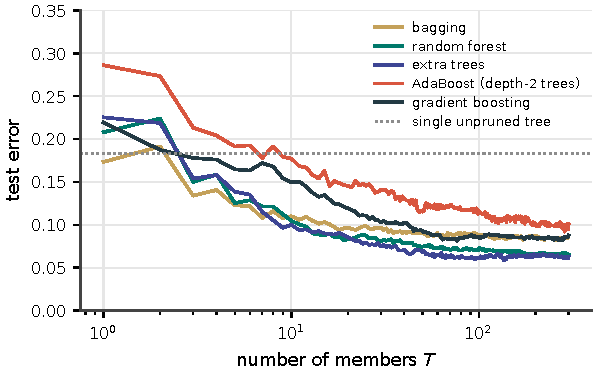
\includegraphics[width=0.76\textwidth]{ch02/ensemble_size}
\caption{Test error as a function of the number of members on a synthetic problem with 1500
training examples. The dotted line is a single unpruned tree.}
\label{fig:ensemblesize}
\end{figure}

\subsection{Decorate}

\emph{Decorate\index{Decorate|textbf}} \citep{melville2003constructing} generates diversity\index{diversity} explicitly by adding
\emph{artificial} training examples. In each iteration it generates a number of artificial
examples (a fraction of the size of the training set) from a simple model of the data
distribution, and labels them so that they \emph{differ} from the predictions of the current
ensemble. A new member is trained on the original data plus the artificial examples, and it is
kept only if it does not increase the training error of the ensemble: poor models are not
included. The probabilities of the members are averaged. The original Decorate experiments reported higher accuracy than
the base classifier and than bagging\index{bagging}, and gains over boosting in several small-sample settings, which should be
verified for the task at hand.

% ---------------------------------------------------------------------
\section{Hybrid approaches}\label{sec:hybrid}

Hybrid methods combine models learned with \emph{different} techniques. Different learning
biases produce naturally diverse models: a linear model, a nearest-neighbour\index{k-nearest neighbours@$k$-nearest neighbours} classifier and a
decision tree make different kinds of mistakes.

\subsection{Voting}

The most basic combination of heterogeneous models is voting\index{voting}: each model votes and the class
with most votes wins (\emph{hard} voting), or the probabilities are averaged (\emph{soft}
voting). Diversity\index{diversity} is generated implicitly, by the differences between the techniques. The
drawback of uniform voting is that bad models have the same importance as good ones, so voting
heterogeneous models often gives disappointing results unless all of them are reasonably good.
In \cref{lst:stacking}, hard voting of four models is barely better than the best of them
(accuracy 0.863 against 0.862), and soft voting, which uses the confidence of the members, does
a little better (0.871).

\subsection{Stacking}

\emph{Stacking\index{stacking|textbf}} (stacked generalisation\index{generalisation}, \citealp{wolpert1992stacked}) learns how to combine
the models. It uses two levels of models (\cref{fig:stacking}): the \emph{base models}
(level~0), usually learned with different techniques, and a \emph{metamodel} (level~1),
trained to optimise the fusion\index{fusion of models} of the base models' outputs. The inputs of the metamodel are the
predictions of the base models.

The key to stacking is to avoid overfitting: if the metamodel were trained on predictions that
the base models make on their own training data, it would learn to trust the models that overfit
most. The metamodel must be trained with \emph{fresh} data, that is, with predictions on
examples the base models have not seen. With enough data a separate validation set can be used;
more efficiently, the base models produce \emph{out-of-fold} predictions by cross-validation\index{cross-validation},
and are finally refitted on all the data (\cref{alg:stacking}). \citet{ting1999issues} showed
that stacking works best when the base models provide class probabilities (rather than crisp
labels) and the metamodel is a simple model such as a linear or logistic regression\index{logistic regression}. A
theoretical justification of cross-validated stacking, under the name of \emph{super learner},
was given by \citet{vanderlaan2007super}.

\begin{figure}[htbp]
\centering
\begin{tikzpicture}[font=\scriptsize\sffamily,
  box/.style={draw=edmnavy,fill=edmnavy!6,rounded corners=2pt,minimum height=6mm,align=center},
  mod/.style={draw=edmteal,fill=edmteal!10,rounded corners=2pt,minimum width=19mm,minimum height=6mm,align=center},
  meta/.style={draw=edmcoral,fill=edmcoral!10,rounded corners=2pt,minimum height=9mm,align=center},
  arr/.style={-{Stealth[length=1.8mm]},edmnavy}]
  \node[box,minimum width=14mm,minimum height=17mm] (d) at (0,0) {training\\data\\$(x_i,y_i)$};
  \node[mod] (m1) at (2.7,1.1) {neural network};
  \node[mod] (m2) at (2.7,0) {decision tree};
  \node[mod] (m3) at (2.7,-1.1) {SVM};
  \foreach \i in {1,2,3} \draw[arr] (d.east) -- (m\i.west);
  \node[box,text width=33mm,minimum height=17mm] (z) at (6.5,0)
       {meta-features (out-of-fold)\\[2pt]$z_i=\bigl(\hat p_1(x_i),\hat p_2(x_i),\hat p_3(x_i)\bigr)$};
  \foreach \i in {1,2,3} \draw[arr] (m\i.east) -- (z.west);
  \node[meta] (mm) at (10.1,0) {metamodel\\(e.g.\ logistic\\regression)};
  \draw[arr] (z) -- (mm);
  \node (pred) at (12.4,0) {prediction};
  \draw[arr] (mm) -- (pred);
  \node[text=edmteal!70!black] at (2.7,1.85) {level 0: base models};
  \node[text=edmcoral] at (10.1,0.95) {level 1};
\end{tikzpicture}
\caption{Stacking. The base models, usually learned with different techniques, produce
predictions that become the inputs of a metamodel. To avoid overfitting, the metamodel is
trained on out-of-fold (cross-validated) predictions.}
\label{fig:stacking}
\end{figure}

\begin{algorithm}[htbp]
\caption{Stacking with cross-validated meta-features}\label{alg:stacking}
\begin{algorithmic}[1]
\Require training set $D$; base learners $\mathcal A_1,\dots,\mathcal A_M$; metalearner $\mathcal B$; $K$ folds
\State split $D$ into folds $F_1,\dots,F_K$
\For{$k=1,\dots,K$}
  \For{$m=1,\dots,M$}
    \State $h_m^{(-k)}\gets\mathcal A_m(D\setminus F_k)$
    \State $z_{im}\gets h_m^{(-k)}(x_i)$ for every $x_i\in F_k$ \Comment{out-of-fold predictions}
  \EndFor
\EndFor
\State $g\gets\mathcal B\bigl(\{(z_i,y_i)\}_{i=1}^{n}\bigr)$ \Comment{train the metamodel}
\State $h_m\gets\mathcal A_m(D)$ for $m=1,\dots,M$ \Comment{refit the base models on all the data}
\State \Return $H(x)=g\bigl(h_1(x),\dots,h_M(x)\bigr)$
\end{algorithmic}
\end{algorithm}

\begin{pylisting}[label={lst:stacking}]{Base models, hard and soft voting, and stacking (5-fold CV)}
from sklearn.datasets import make_classification
from sklearn.ensemble import StackingClassifier, VotingClassifier
from sklearn.linear_model import LogisticRegression
from sklearn.model_selection import StratifiedKFold, cross_validate
from sklearn.naive_bayes import GaussianNB
from sklearn.neighbors import KNeighborsClassifier
from sklearn.pipeline import make_pipeline
from sklearn.preprocessing import StandardScaler
from sklearn.tree import DecisionTreeClassifier

X, y = make_classification(n_samples=2000, n_features=20, n_informative=6, n_redundant=4,
                           flip_y=0.05, class_sep=0.8, random_state=11)
base = [("logistic", make_pipeline(StandardScaler(), LogisticRegression())),
        ("naive Bayes", GaussianNB()),
        ("15-NN", make_pipeline(StandardScaler(), KNeighborsClassifier(15))),
        ("tree", DecisionTreeClassifier(max_depth=6, random_state=0))]
models = dict(base)
models["hard voting"] = VotingClassifier(base, voting="hard")
models["soft voting"] = VotingClassifier(base, voting="soft")
models["stacking"] = StackingClassifier(base, final_estimator=LogisticRegression(), cv=5)
cv = StratifiedKFold(5, shuffle=True, random_state=0)
for name, m in models.items():
    scoring = ["accuracy", "roc_auc"] if hasattr(m, "predict_proba") else ["accuracy"]
    r = cross_validate(m, X, y, cv=cv, scoring=scoring)
    auc = f"{r['test_roc_auc'].mean():.3f}" if "roc_auc" in scoring else "  -  "
    print(f"{name:12s} accuracy={r['test_accuracy'].mean():.3f}  AUC={auc}")
\end{pylisting}
\begin{pyoutput}
logistic     accuracy=0.840  AUC=0.907
naive Bayes  accuracy=0.845  AUC=0.908
15-NN        accuracy=0.862  AUC=0.935
tree         accuracy=0.846  AUC=0.871
hard voting  accuracy=0.863  AUC=  -  
soft voting  accuracy=0.871  AUC=0.935
stacking     accuracy=0.882  AUC=0.942
\end{pyoutput}

In \cref{lst:stacking}, stacking obtains the best accuracy (0.882) and AUC\index{area under the ROC curve (AUC)} (0.942), above every
base model and above both kinds of voting\index{voting}. Its evaluation needs the same care as any other
pipeline: the whole procedure, including the internal cross-validation, must be evaluated on
data that it has not seen (\cref{sec:protocols}).

\subsection{Cascading}

In \emph{cascade generalisation\index{cascading|textbf}\index{generalisation|textbf}} \citep{gama2000cascade} the classifiers are applied
sequentially, and each one extends the representation of the data for the next: the class
probability distribution predicted by a base classifier is added to the original attributes as
new attributes, and the next classifier learns from the extended representation. In the
original proposal this is done locally, inside the nodes of a decision tree: at each node,
base-level classifiers are induced with the examples that reach the node, and their outputs are
added as new candidate attributes for the split. A neural network, a linear regression\index{linear regression} and a
decision tree can thus be chained, each one using the previous models' outputs as additional
features.

The word \emph{cascade} is also used, in computer vision, for a different idea: a sequence of
increasingly complex classifiers in which the early, cheap ones reject the easy negative examples
and only the difficult ones reach the expensive stages. The Viola--Jones face detector
\citep{viola2001rapid} made this kind of cascade famous; its goal is speed, and it is close in
spirit to the delegating\index{delegation} classifiers of \cref{sec:cautious}.

\subsection{Mixtures of experts}

A \emph{mixture of experts\index{mixture of experts|textbf}} \citep{jacobs1991adaptive} generates several experts (classifiers or
regressors) whose outputs are combined through a (generalised) linear rule whose weights depend
on the input: a \emph{gating} model $g$ decides how much to trust each expert for each example,
\begin{equation}
  \bar f(y\mid x)=\sum_{t=1}^{T}g_t(x)\,f_t(y\mid x),\qquad
  g_t(x)=\frac{e^{v_t^{\top}x}}{\sum_{s}e^{v_s^{\top}x}}.
\end{equation}
Experts and gate are trained together, classically with the expectation--maximisation\index{expectation maximisation (EM)} (EM)
algorithm, and both use the input examples, so each expert specialises in a region of the input
space. Several mixtures can be combined in a tree, giving a \emph{hierarchical} mixture of
experts \citep{jordan1994hierarchical}. Mixtures of experts are useful when the experts are
diverse, and the idea has had a spectacular revival in deep learning: \emph{sparse} mixtures of
experts, in which the gate activates only a few experts for each input, allow enormous neural
networks, including several large language models\index{large language model (LLM)}\index{language model}, to be trained and run at a fraction of the
cost of a dense network of the same size \citep{shazeer2017outrageously,fedus2022switch}.

% ---------------------------------------------------------------------
\section{Knowing when not to predict: abstention and delegation}\label{sec:cautious}

Combining models is one way of dealing with their limitations. Another is to let a model admit
them. Deployed systems rarely face only the choice ``predict class $a$ or class $b$'': there is
almost always a third option, \emph{do not decide here and pass the case on}. A fraud detector
sends doubtful transactions to a team of analysts; a triage system refers unclear cases to a
doctor; a content moderation pipeline escalates borderline posts to human reviewers; a cheap
model answers the easy queries and calls an expensive one for the hard ones. This section
studies the two forms of the idea: \emph{abstaining}, where a cautious classifier\index{cautious classifier} says ``I do not
know'' and someone else (often a person) decides, and \emph{delegating\index{delegation|textbf}}, where the classifier
passes the case to another model.

\subsection{The reject option}

Let us add to the possible decisions an extra one, ``unknown'', denoted $\perp$, which has a cost
$c_r$. As in \cref{sec:costs}, the best decision for an example is the one with the lowest
expected cost\index{expected cost}, now with one more option: \emph{abstain\index{abstention|textbf} when every prediction has a higher
expected cost than abstaining}.

\citet{chow1970optimum} derived the optimal rule for the simplest case: errors cost 1, correct
predictions cost 0, and abstaining costs $c_r$ (with $0\leq c_r\leq1/2$). The expected cost of
predicting the most probable class is $1-\max_ip_i$, so, with calibrated probabilities, it is
optimal to abstain whenever
\begin{equation}\label{eq:chow}
  \max_i\,p_i<1-c_r .
\end{equation}
The cheaper abstaining is, the more often the classifier should abstain.

With unequal error costs the reasoning is the same. For two classes, if $p$ is the probability
of the positive class, predicting positive costs $(1-p)\,c_{\mathrm{FP}}$ on average, predicting
negative costs $p\,c_{\mathrm{FN}}$, and abstaining costs $c_r$. Abstaining is optimal when both
predictions are more expensive than abstaining, that is, when
\begin{equation}\label{eq:rejectband}
  \frac{c_r}{c_{\mathrm{FN}}}<p<1-\frac{c_r}{c_{\mathrm{FP}}}.
\end{equation}
The classifier abstains on a band of probabilities that contains the cost threshold
$t^\star=c_{\mathrm{FP}}/(c_{\mathrm{FP}}+c_{\mathrm{FN}})$ of \cref{eq:tstar}; the band is empty, and
abstaining is never worthwhile, when
$c_r\geq c_{\mathrm{FP}}c_{\mathrm{FN}}/(c_{\mathrm{FP}}+c_{\mathrm{FN}})$. With more classes, the cost
matrix\index{cost matrix} simply gets an extra row for $\perp$.

\begin{example}{When abstaining is the best decision}{costcautious}
A three-class problem has the following costs (rows: decision; columns: actual class; negative
values are benefits). Abstaining costs nothing.
\begin{center}\small
\begin{tabular}{@{}lrrr@{}}
\toprule
{\footnotesize decision\,\textbackslash\,actual} & $a$ & $b$ & $c$\\
\midrule
$a$ & $-2.5$ & $4$ & $2$\\
$b$ & $2.1$ & $-3.5$ & $0$\\
$c$ & $1.2$ & $1.3$ & $-4$\\
$\perp$ & $0$ & $0$ & $0$\\
\bottomrule
\end{tabular}
\end{center}
For an example with probabilities $(0.40,0.35,0.25)$ the expected costs of predicting $a$, $b$,
$c$ and $\perp$ are $0.9$, $-0.385$, $-0.065$ and $0$: the best decision is $b$, although $a$ is
more probable. For $(0.50,0.28,0.22)$ they are $0.31$, $0.07$, $0.084$ and $0$: every prediction
has a positive expected cost, and the best decision is to abstain, although $a$ has a
probability of 0.5 (part (a) of \cref{lst:costcautious}).
\end{example}

\subsection{Evaluating cautious classifiers}

A \emph{cautious classifier\index{cautious classifier|textbf}} \citep{ferri2004cautious} adds the class $\perp$ to the set of
original classes $C$. It must find a compromise between reducing the number of misclassified
examples (\emph{error}) and reducing the number of unclassified examples (\emph{abstention\index{abstention|textbf}}):
abstaining always is never wrong and never useful. Its confusion matrix\index{confusion matrix} has an extra row for
$\perp$. If $M(i,j)$ counts the examples predicted as $i\in C\cup\{\perp\}$ whose actual class is
$j\in C$, and $\mathit{Card}$ is the total number of examples:
\begin{align}
  \text{Coverage}&=\frac{\sum_{i\in C,\,j\in C}M(i,j)}{\mathit{Card}}, &
  \text{Abstention}&=\frac{\sum_{j\in C}M(\perp,j)}{\mathit{Card}},\\
  \text{Accuracy}&=\frac{\sum_{i\in C}M(i,i)}{\sum_{i\in C,\,j\in C}M(i,j)}, &
  \text{Error}&=\frac{\sum_{i,j\in C,\,i\neq j}M(i,j)}{\mathit{Card}}.
\end{align}
The accuracy is computed on the \emph{covered} examples, whereas the error is relative to all of
them. They satisfy $\text{Coverage}+\text{Abstention}=1$ and
$\text{Accuracy}\times\text{Coverage}=\text{Coverage}-\text{Error}$.

\begin{example}{Evaluating a cautious classifier}{cautious}
A cautious classifier with classes $\{a,b,c\}$ produces this confusion matrix on 100 test
examples (rows: predicted; columns: actual):
\begin{center}\small
\begin{tabular}{@{}lccc@{}}
\toprule
{\footnotesize pred.\,\textbackslash\,actual} & $a$ & $b$ & $c$\\
\midrule
$a$ & 19 & 1 & 2\\
$b$ & 0 & 30 & 0\\
$c$ & 0 & 1 & 38\\
$\perp$ & 1 & 2 & 6\\
\bottomrule
\end{tabular}
\end{center}
It classifies 91 examples and abstains on 9: coverage\index{coverage} 0.91 and abstention 0.09. Of the 91
classified examples, 87 are correct: accuracy $87/91=0.956$. The four mistakes give an error of
$4/100=0.04$, and indeed $0.956\times0.91=0.87=0.91-0.04$ (\cref{lst:cautious}).
\end{example}

A single matrix describes one operating point\index{operating point}. The quality of a cautious classifier is the whole
trade-off, which is shown in an \emph{accuracy\index{accuracy|textbf} response graph}: the accuracy on the covered
examples against the abstention, obtained by abstaining on increasingly large fractions of the
least confident examples (\cref{fig:cautious}a). The literature on \emph{selective
classification} shows the same information as a \emph{risk--coverage\index{risk--coverage curve|textbf}} curve, the error on the
covered examples against the coverage \citep{elyaniv2010foundations,geifman2017selective}. Two
summaries are useful: the accuracy at the level of abstention that the application can afford
(say, 20\%), and the \emph{area under the risk--coverage curve} (AURC\index{AURC}), the average error of the
$k$ most confident predictions over all values of $k$ \citep{geifman2019bias}; lower is better.

What makes a good cautious classifier is not its accuracy but whether its confidence
\emph{ranks its own mistakes}: the examples it is least sure about must be the ones it would get
wrong. This can be measured directly as the AUC of the confidence for separating correct from
incorrect predictions (\cref{sec:roc}), and it depends on the quality of the probabilities
(\cref{sec:calibration}). In \cref{fig:cautious}a, the decision tree is the most accurate
classifier when it must classify everything (0.824), but its confidence, based on a few leaf
frequencies, ranks its errors poorly (AUC 0.648, against 0.700 for logistic regression and 0.724
for naive Bayes\index{naive Bayes}): its curve flattens and then falls, and it has the worst AURC (0.147). Naive
Bayes has the best AURC (0.101) and becomes the most accurate model above 50\% abstention. The tree
produces only a few distinct confidences, so the order of the examples within ties changes its curve
and its AURC: a tie policy must be stated, for instance averaging over random orders. Which
model is best depends on how much abstention the application can tolerate.

Naive Bayes deserves a second look, because \cref{sec:calibration} showed that its probabilities are badly
calibrated. There is no contradiction: abstaining on a fixed share of the least confident cases, as AURC and
delegation\index{delegation} do, only needs a confidence that \emph{ranks} the errors well (any strictly increasing transformation of
it gives the same curve), whereas abstaining with cost-based thresholds, as the window rule\index{window rule} below does, needs
probabilities that are \emph{calibrated\index{calibration|textbf}}. Part~(c) of \cref{lst:costcautious} applies the cost-matched window rule
to naive Bayes on the same data: uncalibrated, it abstains on 22.8\% of the test cases at a mean cost of 0.326;
after isotonic\index{calibration!isotonic regression} calibration it abstains on 36.3\% at a mean cost of 0.312.

\begin{pylisting}[label={lst:cautious}]{Evaluation of a cautious classifier, and how well three models rank their own errors}
import numpy as np
from sklearn.datasets import make_classification
from sklearn.linear_model import LogisticRegression
from sklearn.metrics import roc_auc_score
from sklearn.model_selection import train_test_split
from sklearn.naive_bayes import GaussianNB
from sklearn.tree import DecisionTreeClassifier

# (a) Rows = predicted a, b, c and "unknown"; columns = actual a, b, c
M = np.array([[19, 1, 2], [0, 30, 0], [0, 1, 38], [1, 2, 6]])
card, covered, hits = M.sum(), M[:3].sum(), np.trace(M[:3])
print(f"coverage={covered / card:.2f}  abstention={M[3].sum() / card:.2f}  "
      f"accuracy={hits / covered:.3f}  error={(covered - hits) / card:.2f}")

# (b) Does the confidence of each model rank its own mistakes?
X, y = make_classification(n_samples=4000, n_features=20, n_informative=6, n_redundant=4,
                           flip_y=0.05, class_sep=0.8, random_state=5)
X_tr, X_te, y_tr, y_te = train_test_split(X, y, test_size=0.5, random_state=0)
for name, m in [("logistic", LogisticRegression(max_iter=1000)),
                ("naive Bayes", GaussianNB()),
                ("tree (depth 6)", DecisionTreeClassifier(max_depth=6, random_state=0))]:
    P = m.fit(X_tr, y_tr).predict_proba(X_te)
    conf, correct = P.max(axis=1), P.argmax(axis=1) == y_te
    ok = correct[np.argsort(-conf, kind="stable")]            # most confident first
    risk = 1 - np.cumsum(ok) / np.arange(1, len(ok) + 1)      # error of the top-k
    acc20 = 1 - risk[int(0.8 * len(ok)) - 1]                  # with 20% abstention
    auc = roc_auc_score(correct, conf)                        # confidence vs correctness
    print(f"{name:14s} acc={correct.mean():.3f}  acc@20%abst={acc20:.3f}  "
          f"AURC={risk.mean():.3f}  AUC(conf)={auc:.3f}")
\end{pylisting}
\begin{pyoutput}
coverage=0.91  abstention=0.09  accuracy=0.956  error=0.04
logistic       acc=0.766  acc@20%abst=0.814  AURC=0.129  AUC(conf)=0.700
naive Bayes    acc=0.792  acc@20%abst=0.843  AURC=0.101  AUC(conf)=0.724
tree (depth 6) acc=0.824  acc@20%abst=0.874  AURC=0.147  AUC(conf)=0.648
\end{pyoutput}

\subsection{From probabilistic to cautious classifiers}

Any probabilistic classifier $f$, which assigns to each example a vector of $|C|$ probabilities
$p_i$, can be turned into a cautious classifier\index{cautious classifier}. Following \citet{ferri2004cautious}, define a
\emph{class bias} $K=\{k_i\}_{i=1}^{|C|}$ with $\sum_ik_i=1$, and a \emph{window size}
$w\in[0,1]$:
\begin{center}
\fbox{\begin{minipage}{0.86\textwidth}
\textbf{Decision rule\index{decision rules|textbf}} (given $K$ and $w$). For each class $i$, compute the threshold
$\tau_i=(1-k_i)\,w+k_i$. If some $p_i\geq\tau_i$, predict $\argmax_i\,(p_i/\tau_i)$ among those
classes; otherwise predict $\perp$.
\end{minipage}}
\end{center}
With $w=0$ the thresholds are the class biases themselves and the classifier never abstains\index{abstention}: with
a uniform $K$ it predicts the most probable class, and with a non-uniform $K$ it shifts the
decision towards some classes, as a cost-sensitive\index{cost-sensitive learning} threshold does. As $w$ grows, the thresholds
move towards 1 and the classifier abstains more and more; with $w=1$ it only predicts when it is
completely sure.

For two classes the rule has a simple geometry. If $k$ is the bias of the positive class, it
predicts positive when $p\geq k+(1-k)\,w$, negative when $p\leq k\,(1-w)$, and abstains in
between,
\begin{equation}\label{eq:windowband}
  k\,(1-w)<p<k+(1-k)\,w,
\end{equation}
a \emph{window} around $k$ whose width grows with $w$. Comparing it with the optimal band of
\cref{eq:rejectband} gives a remarkable result. Take $k=t^\star$ and
\begin{equation}\label{eq:wstar}
  w^\star=1-\frac{c_r\,(c_{\mathrm{FP}}+c_{\mathrm{FN}})}{c_{\mathrm{FP}}\,c_{\mathrm{FN}}}.
\end{equation}
Then $k(1-w^\star)=\frac{c_{\mathrm{FP}}}{c_{\mathrm{FP}}+c_{\mathrm{FN}}}\cdot
\frac{c_r(c_{\mathrm{FP}}+c_{\mathrm{FN}})}{c_{\mathrm{FP}}c_{\mathrm{FN}}}=\frac{c_r}{c_{\mathrm{FN}}}$
and, in the same way, $k+(1-k)\,w^\star=1-(1-k)(1-w^\star)=1-\frac{c_r}{c_{\mathrm{FP}}}$: the two
bands coincide.

\begin{keyidea}
For two classes, the window rule\index{window rule} with the class bias matched to the error costs,
$K=(1-t^\star,t^\star)$, and the window $\max(0,w^\star)$, with $w^\star$ from \cref{eq:wstar}, \emph{is} the
optimal cost-sensitive reject rule for positive error costs, given the probabilities it receives; when
$c_r\geq c_{\mathrm{FP}}c_{\mathrm{FN}}/(c_{\mathrm{FP}}+c_{\mathrm{FN}})$ the window is 0 and abstaining never pays. Chow's rule is the special case of equal costs: $K=(0.5,0.5)$ and
$w^\star=1-2c_r$. The class bias $K$ encodes the costs of the errors; the window $w$ encodes the
cost of abstaining.
\end{keyidea}

For instance, with $c_{\mathrm{FP}}=1$, $c_{\mathrm{FN}}=4$ and $c_r=0.5$, the cost threshold is
$t^\star=0.2$, the window is $w^\star=1-0.5\cdot5/4=0.375$, and both rules abstain exactly when
$0.125<p<0.5$; part (b) of \cref{lst:costcautious} checks that they take the same decision for
every probability. \Cref{fig:cautious}b shows what is at stake on a problem with 20\% of positives.
With a uniform $K$ and $w=0$ the logistic regression uses the threshold 0.5, ignores the costs,
and costs 0.537 per example; with the cost-matched $K$ it costs 0.386 without abstaining at all.
As $w$ grows both curves fall, because abstaining (0.5) is cheaper than many risky predictions;
the cost-matched curve stays below the uniform one, and its minimum is reached at $w^\star$ (the
star: 42\% of abstentions and a cost of 0.327 per example), where it makes exactly the decisions
of the optimal rule. With more than two classes the window rule is not always identical to the
optimal one, but $K$ and $w$ keep the same interpretation.

\begin{figure}[htbp]
\centering
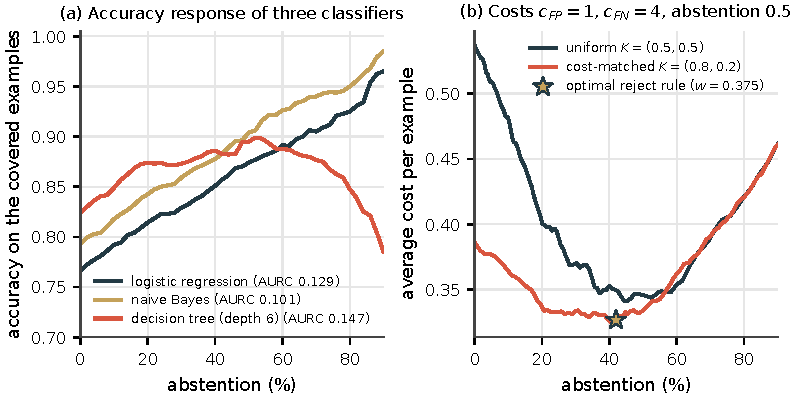
\includegraphics[width=\textwidth]{ch02/cautious}
\caption{(a) Accuracy response graphs of three classifiers (2000 test examples); the AURC
summarises each curve. (b) Average cost of a logistic regression turned into a cautious
classifier with the window rule, for a uniform and a cost-matched class bias, as the window
grows; the star is the optimal reject rule.}
\label{fig:cautious}
\end{figure}

\begin{pylisting}[label={lst:costcautious}]{Expected costs with an abstention option, and the window rule as the optimal reject rule}
import numpy as np
from sklearn.calibration import CalibratedClassifierCV
from sklearn.datasets import make_classification
from sklearn.model_selection import train_test_split
from sklearn.naive_bayes import GaussianNB

# (a) Costs: rows = decision (a, b, c, unknown), columns = actual class (a, b, c)
C = np.array([[-2.5,  4.0,  2.0],
              [ 2.1, -3.5,  0.0],
              [ 1.2,  1.3, -4.0],
              [ 0.0,  0.0,  0.0]])
decisions = np.array(["a", "b", "c", "unknown"])
for p in ([0.40, 0.35, 0.25], [0.50, 0.28, 0.22]):
    ec = C @ np.array(p)                       # expected cost of each decision
    print(f"p={p}  expected costs={ec.round(3)}  ->  {decisions[ec.argmin()]}")

# (b) Two classes: the window rule with a cost-matched K is the optimal reject rule
def cautious_predict(P, K, w):
    tau = (1 - np.asarray(K)) * w + np.asarray(K)      # one threshold per class
    ok = P >= tau
    pred = np.where(ok, P / tau, -np.inf).argmax(axis=1)
    pred[~ok.any(axis=1)] = -1                          # -1 means "unknown"
    return pred

c_fp, c_fn, c_r = 1.0, 4.0, 0.5
t = c_fp / (c_fp + c_fn)                                # cost threshold t*
w = 1 - c_r * (c_fp + c_fn) / (c_fp * c_fn)
p = np.linspace(0.0005, 0.9995, 1000)                   # P(positive)
window = cautious_predict(np.c_[1 - p, p], K=(1 - t, t), w=w)
cost = np.c_[p * c_fn, (1 - p) * c_fp, np.full_like(p, c_r)]   # predict 0, 1, abstain
bayes = np.array([0, 1, -1])[cost.argmin(axis=1)]
print(f"t*={t:.2f}  w={w:.3f}  identical decisions: {np.mean(window == bayes):.3f}")
print(f"abstains for p in [{p[window == -1].min():.4f}, {p[window == -1].max():.4f}]")

# (c) Data of Listing 2.9: ranking errors well is not enough, the window needs calibration
X, y = make_classification(n_samples=4000, n_features=20, n_informative=6, n_redundant=4,
                           flip_y=0.05, class_sep=0.8, random_state=5)
X_tr, X_te, y_tr, y_te = train_test_split(X, y, test_size=0.5, random_state=0)
for name, m in [("naive Bayes", GaussianNB()),
                ("naive Bayes + isotonic",
                 CalibratedClassifierCV(GaussianNB(), method="isotonic"))]:
    p1 = m.fit(X_tr, y_tr).predict_proba(X_te)[:, 1]
    d = cautious_predict(np.c_[1 - p1, p1], K=(1 - t, t), w=w)
    loss = np.where(d == -1, c_r, np.where(d == 1, (y_te == 0) * c_fp, (y_te == 1) * c_fn))
    print(f"{name:23s} abstains {np.mean(d == -1):.3f}  mean cost {loss.mean():.3f}")
\end{pylisting}
\begin{pyoutput}
p=[0.4, 0.35, 0.25]  expected costs=[ 0.9   -0.385 -0.065  0.   ]  ->  b
p=[0.5, 0.28, 0.22]  expected costs=[0.31  0.07  0.084 0.   ]  ->  unknown
t*=0.20  w=0.375  identical decisions: 1.000
abstains for p in [0.1255, 0.4995]
naive Bayes             abstains 0.228  mean cost 0.326
naive Bayes + isotonic  abstains 0.363  mean cost 0.312
\end{pyoutput}

Conformal prediction\index{conformal prediction} (\cref{sec:other}) offers another way of deciding when to abstain, with a
different guarantee: compute prediction sets with coverage\index{coverage} $1-\alpha$ and abstain whenever the
set does not contain exactly one label: two or more labels signal ambiguity\index{ambiguity decomposition}, and an empty set signals that
no label is plausible, as for an input unlike the calibration data. In \cref{lst:conformalabst}, 90\% prediction sets cover 90.1\%
of the test examples; 67.0\% of them contain a single label, with an accuracy of 0.853; the other
33.0\% contain both labels, and no set is empty with this $\alpha$, although empty sets become possible as $\alpha$
grows. The guarantee concerns the coverage of the sets,
not the accuracy of the single-label predictions.

\begin{pylisting}[label={lst:conformalabst}]{Abstaining when a conformal prediction set is not a single label}
import numpy as np
from sklearn.datasets import make_classification
from sklearn.linear_model import LogisticRegression
from sklearn.model_selection import train_test_split

X, y = make_classification(n_samples=6000, n_features=20, n_informative=6, n_redundant=4,
                           flip_y=0.05, class_sep=0.8, random_state=5)
X_tr, X_rest, y_tr, y_rest = train_test_split(X, y, test_size=2 / 3, random_state=0)
X_cal, X_te, y_cal, y_te = train_test_split(X_rest, y_rest, test_size=0.5, random_state=1)
model = LogisticRegression(max_iter=1000).fit(X_tr, y_tr)

alpha = 0.1                                                  # 90% prediction sets
s_cal = 1 - model.predict_proba(X_cal)[np.arange(len(y_cal)), y_cal]
k = int(np.ceil((len(y_cal) + 1) * (1 - alpha)))      # rank of the conformal quantile
q = np.inf if k > len(y_cal) else np.sort(s_cal)[k - 1]
sets = 1 - model.predict_proba(X_te) <= q                    # label j in the set?
size = sets.sum(axis=1)
one = size == 1                                              # predict; otherwise abstain
covered = np.mean(sets[np.arange(len(y_te)), y_te])
print(f"set coverage={covered:.3f} (target {1 - alpha:.2f})")
print(f"single-label sets={one.mean():.3f}  abstain: two labels={np.mean(size == 2):.3f}  "
      f"empty={np.mean(size == 0):.3f}")
acc_one = np.mean(sets[one].argmax(axis=1) == y_te[one])
print(f"accuracy on single-label sets={acc_one:.3f}")
\end{pylisting}
\begin{pyoutput}
set coverage=0.901 (target 0.90)
single-label sets=0.670  abstain: two labels=0.330  empty=0.000
accuracy on single-label sets=0.853
\end{pyoutput}

\subsection{Delegating classifiers}

Abstaining is not always an option: a bank must eventually accept or reject the loan. A
\emph{delegating\index{delegation|textbf} classifier} \citep{ferri2004delegating} delegates the difficult or uncertain
predictions to other, possibly more specialised, classifiers. In the \emph{two-step scenario}, a
first classifier is learned from all the training data; it keeps the examples on which it is
confident and delegates the rest, and a second classifier is learned from the delegated training
examples only. At prediction time, each new example is classified by the first classifier if its
confidence exceeds the threshold, and passed to the second one otherwise. In the \emph{iterated
scenario}, an arbitrary number of classifiers are chained in the same way. In the \emph{round
rebound\index{round rebound|textbf}} variant (\cref{fig:delegation}), the cases that are very difficult for the second level,
those on which it is not confident either, come back to the first level, which makes the final
prediction.

\begin{figure}[htbp]
\centering
\begin{tikzpicture}[font=\scriptsize\sffamily,
  box/.style={draw=edmnavy,fill=edmnavy!6,rounded corners=2pt,minimum height=7mm,align=center},
  mod/.style={draw=edmteal,fill=edmteal!10,rounded corners=2pt,minimum width=17mm,minimum height=7mm,align=center},
  dec/.style={diamond,draw=edmcoral,fill=edmcoral!8,aspect=2.3,inner sep=1pt,align=center},
  arr/.style={-{Stealth[length=1.8mm]},edmnavy}]
  \node[box] (x) at (0,0) {new\\example $x$};
  \node[mod] (c1) at (2.2,0) {classifier 1};
  \node[dec] (q1) at (4.6,0) {confident?\\$c_1(x)>\theta_1$};
  \node[box,minimum width=36mm] (p1) at (8.6,1.25) {prediction of classifier 1};
  \node[mod] (c2) at (7.4,-1.25) {classifier 2};
  \node[dec] (q2) at (9.9,-1.25) {confident?\\$c_2(x)>\theta_2$};
  \node[box] (p2) at (12.7,-1.25) {prediction of\\classifier 2};
  \draw[arr] (x) -- (c1);
  \draw[arr] (c1) -- (q1);
  \draw[arr] (q1.north) |- node[above,pos=0.75] {yes} (p1.west);
  \draw[arr] (q1.south) |- node[below,pos=0.75] {no: delegate} (c2.west);
  \draw[arr] (c2) -- (q2);
  \draw[arr] (q2) -- node[above] {yes} (p2);
  \draw[arr,dashed,edmcoral] (q2.north) -- node[right,pos=0.45,text=edmcoral,align=left]
       {no: round\\rebound} (q2.north |- p1.south);
\end{tikzpicture}
\caption{Two-step delegation with round rebound. The second classifier is trained on the
examples that the first one delegates, so it specialises in the difficult cases; the cases on
which it is not confident either go back to the first level (dashed arrow).}
\label{fig:delegation}
\end{figure}

Delegation serves two different purposes, depending on the second level:
\begin{itemize}
  \item \emph{specialisation}: as in the original proposal, the second classifier is learned
        from the delegated examples and becomes an expert in the difficult region. Each
        classifier learns from fewer examples than the previous one, which makes delegation
        \emph{efficient}; every prediction is made by a single classifier, which keeps the system
        \emph{comprehensible\index{comprehensibility|textbf}} (with decision trees, it is a short list of trees with confidence
        conditions); and the parts of the system that lead to delegation can be removed to
        simplify it;
  \item \emph{efficiency} (a \emph{cascade\index{cascading|textbf}}): the second level is a stronger but more expensive
        model, trained on all the data, and the first level answers the easy cases cheaply. The
        aim is to obtain most of the accuracy of the expensive model while calling it for only a
        fraction of the examples.
\end{itemize}

\Cref{fig:graphdelegation} and \cref{lst:delegation} compare the variants, with a decision tree of
16 leaves as first level. The delegation thresholds are taken from \emph{out-of-fold} confidences
(\cref{sec:protocols}): on its own training data a model is overconfident, so a quantile of those confidences would
delegate fewer new examples than intended. Delegating to a random forest raises the accuracy from 0.803 (the tree
alone) to 0.882, closing three quarters of the gap with the forest (0.908) while calling it for only 717 of the 3000
test examples (24\%, not the nominal 30\%: the tree produces only 16 distinct confidences, so the quantile is
coarse), and every prediction that is not delegated can be explained by the small tree. A specialist tree trained on
the delegated examples reaches 0.842 (and 0.850 at best); its curve is irregular because each delegation threshold
produces a different training set for the specialist. Round rebound returns 227 of the 717 delegated cases to the
first tree and leaves the accuracy unchanged here (0.842): the cases that bounce back are, by construction, those the
first tree had already found difficult, so it is no better than the specialist on them. Rebound pays off only when
the first level remains competent on part of the region it delegates. As with every design choice in this book, the
variant must be validated on data (Exercise~\ref{exr2:rebound}). The delegation rate is measured on the test data,
because no quantile estimated during training guarantees the same rate in deployment\index{deployment}, and the time actually saved
must be measured as well, since the cost of the second level depends on the hardware and on batching.

\begin{figure}[htbp]
\centering
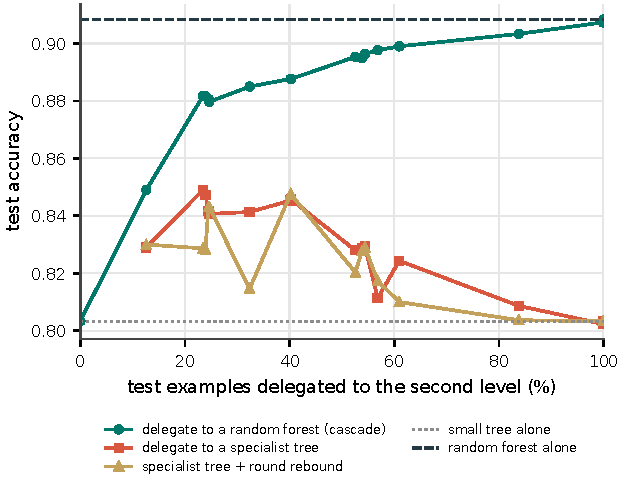
\includegraphics[width=0.78\textwidth]{ch02/delegation}
\caption{Accuracy of three delegation schemes as a function of the fraction of test examples sent
to the second level. The first level is a decision tree with 16 leaves; the cascade delegates to
a random forest of 200 trees trained on all the data.}
\label{fig:graphdelegation}
\end{figure}

\begin{pylisting}[label={lst:delegation}]{Two-step delegation: specialist, round rebound and cascade}
import numpy as np
from sklearn.datasets import make_classification
from sklearn.ensemble import RandomForestClassifier
from sklearn.model_selection import cross_val_predict, train_test_split
from sklearn.tree import DecisionTreeClassifier

class DelegatingClassifier:
    """Two-step delegation (after Ferri, Flach and Hernandez-Orallo, 2004).
    The first model delegates its least confident fraction of the examples. If
    specialise=True the second model is trained only on the delegated examples; if
    rebound > 0, it returns its own least confident fraction to the first model."""
    def __init__(self, first, second, delegate=0.3, specialise=True, rebound=0.0):
        self.first, self.second, self.delegate = first, second, delegate
        self.specialise, self.rebound = specialise, rebound

    def fit(self, X, y):
        # thresholds from out-of-fold confidences: on its own training data a model
        # is overconfident, so training quantiles would delegate too few new examples
        oof = lambda m, A, b: cross_val_predict(m, A, b, cv=5, method="predict_proba")
        conf = oof(self.first, X, y).max(axis=1)
        self.first.fit(X, y)
        self.t1_ = np.quantile(conf, self.delegate)
        hard = conf <= self.t1_                               # delegated examples
        Xs, ys = (X[hard], y[hard]) if self.specialise else (X, y)
        self.second.fit(Xs, ys)
        if self.rebound:
            conf2 = oof(self.second, Xs, ys).max(axis=1)
            self.t2_ = np.quantile(conf2 if self.specialise else conf2[hard], self.rebound)
        else:
            self.t2_ = -np.inf
        return self

    def predict(self, X):
        """The first model sees every example, the second only the delegated ones."""
        P1 = self.first.predict_proba(X)
        pred = self.first.classes_[P1.argmax(axis=1)]
        idx = np.flatnonzero(P1.max(axis=1) <= self.t1_)          # delegated examples
        self.n_second_ = len(idx)
        if len(idx):
            P2 = self.second.predict_proba(X[idx])
            take = P2.max(axis=1) > self.t2_                       # else: round rebound
            pred[idx[take]] = self.second.classes_[P2[take].argmax(axis=1)]
        return pred

X, y = make_classification(n_samples=6000, n_features=10, n_informative=6, n_redundant=2,
                           flip_y=0.03, class_sep=1.0, random_state=8)
X_tr, X_te, y_tr, y_te = train_test_split(X, y, test_size=0.5, random_state=0)
tree = lambda: DecisionTreeClassifier(max_depth=4, random_state=0)
forest = lambda: RandomForestClassifier(200, random_state=0)
systems = {"small tree alone": tree(),
           "specialist (two small trees)": DelegatingClassifier(tree(), tree()),
           "specialist + round rebound": DelegatingClassifier(tree(), tree(), rebound=0.3),
           "cascade: small tree -> forest":
               DelegatingClassifier(tree(), forest(), specialise=False),
           "random forest alone": forest()}
for name, m in systems.items():
    acc = np.mean(m.fit(X_tr, y_tr).predict(X_te) == y_te)
    calls = ""
    if hasattr(m, "n_second_"):                       # delegating systems
        calls = f"  (second model: {m.n_second_} of {len(y_te)})"
    print(f"{name:30s} accuracy={acc:.3f}{calls}")
\end{pylisting}
\begin{pyoutput}
small tree alone               accuracy=0.803
specialist (two small trees)   accuracy=0.842  (second model: 717 of 3000)
specialist + round rebound     accuracy=0.842  (second model: 717 of 3000)
cascade: small tree -> forest  accuracy=0.882  (second model: 717 of 3000)
random forest alone            accuracy=0.908
\end{pyoutput}

\subsection{Delegating to humans and to large models}

When the second level is a person, delegation\index{delegation} becomes \emph{learning to defer}
\citep{madras2018predict,mozannar2020consistent}. The decision to defer should depend not only
on the confidence of the model but also on how good the human is on each kind of case: a model
should defer the cases that the human is likely to get right and it is likely to get wrong, so
the classifier and the deferral rule are trained together to minimise the error of the
human--machine team rather than that of the model alone. Deferring well can also make the whole
system fairer, if the model is less reliable for some groups of people
\citep{madras2018predict}. The same structure appears with large language models\index{large language model (LLM)}: a model
\emph{cascade\index{cascading|textbf}} sends each query to a cheap model first and uses a scoring function to decide
whether to accept its answer or escalate to a more expensive model, which can match the accuracy
of the most expensive model at a much lower cost \citep{chen2023frugalgpt}. The gating network of
a mixture of experts\index{mixture of experts} (\cref{sec:hybrid}) is yet another form of routing.

Evaluating these systems requires the quantities of this section: the accuracy or the cost as a
function of the fraction of delegated cases, and the workload sent to the human team or to the
expensive model. Once the system is deployed, the delegation rate itself is worth monitoring\index{monitoring}
(Unit~6): if a model starts to abstain\index{abstention} or delegate much more often than during validation, the
data have probably changed.

% ---------------------------------------------------------------------
\section{How good are combinations in practice?}\label{sec:performance}

\subsection{Bagging, boosting, randomisation and noise}

\citet{dietterich2000experimental} compared experimentally three methods for constructing
ensembles of decision trees: boosting, bagging\index{bagging} and randomisation\index{randomisation}. In problems without noise,
boosting obtained the best results, and bagging and randomisation were quite similar. In noisy
data sets, however, bagging was the best method, followed by randomisation, and boosting was
the worst. \citet{bauer1999empirical} obtained similar results in a large comparison of voting\index{voting}
methods.

\Cref{fig:noise} reproduces the experiment on synthetic data, flipping\index{attribute flipping} a fraction of the training
labels while testing on clean data. Without noise, AdaBoost\index{AdaBoost} is the most accurate method (0.898,
against 0.893 for the random forest and 0.885 for bagging). With 10\% of noise it has already
fallen behind both (0.848, against 0.888 and 0.870), and with 30\% the gap is large (0.686,
against 0.786 and 0.772). The reason is the exponential loss discussed in \cref{sec:ensembles}:
mislabelled\index{label noise} examples are, by definition, those the ensemble keeps getting wrong, and AdaBoost
keeps increasing their weight until the new members are devoted to fitting the noise.

\begin{figure}[htbp]
\centering
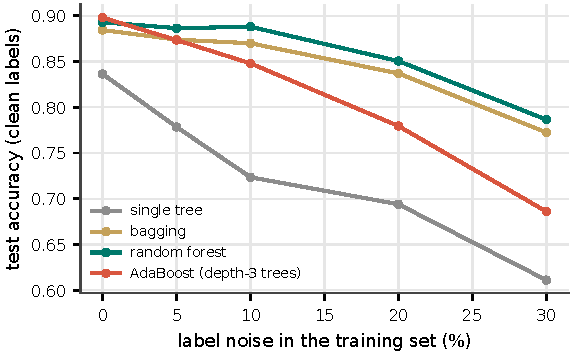
\includegraphics[width=0.72\textwidth]{ch02/noise}
\caption{Test accuracy as a function of the proportion of mislabelled training examples
(average over four synthetic data sets; test labels are clean).}
\label{fig:noise}
\end{figure}

\subsection{Large-scale comparisons}

Several large studies have compared learning algorithms across many problems:
\begin{itemize}
  \item \citet{caruana2004data} compared SVMs, neural networks, decision trees, $k$-NN, bagged
        trees, boosted trees and boosted stumps\index{decision stump} on seven problems with nine metrics, including
        threshold metrics (accuracy, $F$-score, lift\index{lift}), ranking metrics (ROC area, average
        precision\index{average precision}\index{precision}, break-even point) and probability metrics (squared error, cross-entropy\index{log loss},
        calibration). Boosted trees were excellent on the threshold and ranking metrics but
        poorly calibrated; once calibrated with Platt\index{calibration!Platt scaling}'s method (\cref{sec:calibration}) they
        became the best method. Bagged trees performed well and are very easy to train.
  \item \citet{caruana2006empirical} extended the comparison to ten methods and eleven problems:
        calibrated boosted trees were the best method overall, followed closely by random
        forests and then by bagged trees, calibrated SVMs and neural networks.
  \item \citet{fernandezdelgado2014we} evaluated 179 classifiers from 17 families on 121 data
        sets. The best classifier was a random forest, which reached on average 94.1\% of the
        maximum accuracy obtained on each data set, followed by an SVM with Gaussian kernel
        (92.3\%). A few models were clearly better than the rest (random forests, Gaussian SVMs,
        extreme learning machines with Gaussian kernel, C5.0 and averaged neural networks), and
        the random forest family was the best, followed by SVMs, neural networks and boosting
        ensembles. A later re-analysis pointed out problems in the experimental protocol and found that,
        once they were corrected, the differences between the top methods were not
        statistically significant\index{statistical significance} \citep{wainberg2016random}, a good reminder of the lessons of
        Unit~1.
  \item In data science competitions, analyses of the winning solutions show that gradient
        boosting\index{gradient boosting} libraries dominate problems with tabular data, while deep neural networks
        dominate images, audio and text. Recent benchmarks confirm that tree-based ensembles still
        outperform deep learning on typical medium-sized tabular data
        \citep{grinsztajn2022why,shwartzziv2022tabular}.
\end{itemize}

\subsection{A small benchmark}

To close the section, \cref{fig:cdens} compares seven methods on the twelve synthetic data sets
used in \cref{sec:stats}, with the AUC estimated by 5-fold cross-validation and the Friedman and
Nemenyi\index{Nemenyi test} tests. Every ensemble improves dramatically on a single tree (mean AUC 0.856): bagging\index{bagging}
0.922, random forests 0.923, extremely randomised trees\index{extra trees} 0.928, AdaBoost\index{AdaBoost} 0.911, histogram gradient
boosting\index{gradient boosting} 0.923 and stacking\index{stacking} 0.921. The Friedman test\index{Friedman test} rejects the equality of the methods
($\chi^2_F=38.8$, $p<10^{-6}$), but with seven methods and twelve data sets the critical difference\index{critical difference diagram}
is large ($\mathrm{CD}=2.60$): the single tree is significantly worse than all the ensembles except
AdaBoost, and AdaBoost is significantly worse than extra trees, while the differences among the
rest are not significant. With default hyperparameters and small data sets, the main lesson is
that \emph{any} reasonable ensemble is much better than a single tree.

\begin{figure}[htbp]
\centering
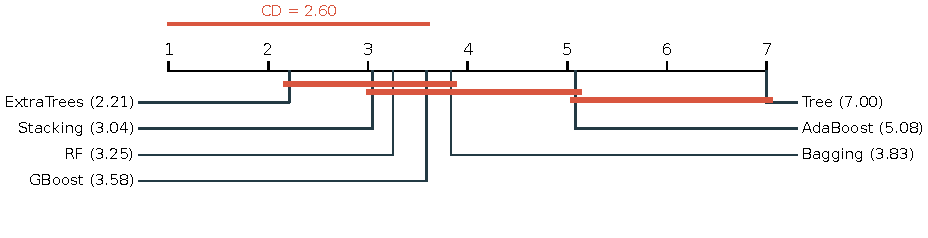
\includegraphics[width=\textwidth]{ch02/cd_ensembles}
\caption{Critical difference diagram of seven methods on twelve data sets (AUC, 5-fold CV;
Nemenyi test, $\alpha=0.05$). Methods joined by a bar are not significantly different.}
\label{fig:cdens}
\end{figure}

% ---------------------------------------------------------------------
\section{Drawbacks}\label{sec:drawbacks}

Ensemble methods classify new examples by a combination of predictions, and this has a price:
\begin{itemize}
  \item \emph{loss of comprehensibility\index{comprehensibility|textbf}}: a single decision tree can be read and checked by an
        expert, but a vote of five hundred trees cannot. The combination can result in a
        complete loss of comprehensibility;
  \item \emph{resources}: a large amount of memory and time is required to construct, store and
        use the ensemble. The prediction throughput\index{throughput} decreases, which is relevant in real-time
        applications and on small devices (Unit~5);
  \item \emph{test costs\index{test costs|textbf}}: to predict the class of an example, most or all of its attributes
        must be measured, which is important when the attributes have costs associated with
        their tests (\cref{sec:costs}).
\end{itemize}

\subsection{Pruning ensembles}

Not all the members of an ensemble are necessary. \emph{Ensemble\index{ensemble|textbf} pruning\index{ensemble pruning|textbf}} selects a subset of the
members that is as good as, or better than, the whole ensemble \citep{margineantu1997pruning}.
\citet{zhou2002ensembling} showed that ``many could be better than all'', and ordering the members
greedily (adding at each step the member that most improves the subensemble on validation data)
and keeping only the first part of the ordering often matches or even improves the full ensemble
with a fraction of the cost \citep{martinezmunoz2009analysis}.

\subsection{Mimetic classifiers and model distillation}

Since ensembles are like black boxes, a natural idea is to use them as \emph{oracles} to train a
single comprehensible\index{comprehensibility} model that copies their behaviour. A \emph{mimetic\index{mimetic classifier|textbf} classifier}
\citep{domingos1997knowledge,estruch2003simple} is built as follows, assuming some information
about the distribution of the features:
\begin{enumerate}
  \item generate a large random data set of unlabelled examples (from the assumed feature
        distributions, or by perturbing the training examples);
  \item label it with the ensemble;
  \item learn an interpretable\index{interpretability} model (a decision tree, a set of rules) from the labelled data.
\end{enumerate}
The mimetic model has as much training data as we want, all labelled consistently by the oracle,
so it can be much better than the same kind of model learned from the original data. Mimetic
classifiers are single, short trees that are comparable in accuracy to bagging\index{bagging} and boosting in
many problems. Their quality is measured by their accuracy and by their \emph{fidelity\index{fidelity|textbf}}, the
proportion of examples on which they agree with the oracle.

\begin{pylisting}[label={lst:mimetic}]{A mimetic tree that imitates a random forest}
import numpy as np
from sklearn.datasets import make_classification
from sklearn.ensemble import RandomForestClassifier
from sklearn.tree import DecisionTreeClassifier, DecisionTreeRegressor

X, y = make_classification(n_samples=4600, n_features=8, n_informative=5, n_redundant=2,
                           flip_y=0.03, class_sep=1.0, random_state=7)
X_tr, y_tr, X_te, y_te = X[:600], y[:600], X[600:], y[600:]
oracle = RandomForestClassifier(n_estimators=300, random_state=0).fit(X_tr, y_tr)

def mimic(oracle, X, n, noise=0.3, max_leaves=32, seed=0, soft=False):
    """Learn a small tree that imitates the oracle on n synthetic examples: from its
    labels (hard targets) or from its probabilities with a regression tree (soft)."""
    rng = np.random.default_rng(seed)
    Xs = X[rng.integers(0, len(X), n)]                          # resample the inputs
    Xs = Xs + rng.normal(0, noise, Xs.shape) * X.std(axis=0)    # and perturb them
    if soft:
        tree = DecisionTreeRegressor(max_leaf_nodes=max_leaves, random_state=0)
        return tree.fit(Xs, oracle.predict_proba(Xs)[:, 1])  # the oracle's probabilities
    tree = DecisionTreeClassifier(max_leaf_nodes=max_leaves, random_state=0)
    return tree.fit(Xs, oracle.predict(Xs))                     # labels of the oracle

def labels(m, X):
    return m.predict(X) if hasattr(m, "classes_") else (m.predict(X) > 0.5).astype(int)

direct = DecisionTreeClassifier(max_leaf_nodes=32, random_state=0).fit(X_tr, y_tr)
ref = oracle.predict(X_te)
for name, m in [("random forest (oracle)", oracle), ("32-leaf tree, original data", direct),
                ("32-leaf mimetic, hard labels", mimic(oracle, X_tr, n=20000)),
                ("32-leaf mimetic, soft targets", mimic(oracle, X_tr, n=20000, soft=True))]:
    pred = labels(m, X_te)
    print(f"{name:29s} accuracy={np.mean(pred == y_te):.3f}  "
          f"fidelity={np.mean(pred == ref):.3f}")
\end{pylisting}
\begin{pyoutput}
random forest (oracle)        accuracy=0.889  fidelity=1.000
32-leaf tree, original data   accuracy=0.830  fidelity=0.896
32-leaf mimetic, hard labels  accuracy=0.859  fidelity=0.922
32-leaf mimetic, soft targets accuracy=0.833  fidelity=0.908
\end{pyoutput}

In \cref{lst:mimetic}, a tree with 32 leaves learned from the original 600 examples has an
accuracy of 0.830; the same kind of tree learned from 20,000 examples labelled by a random forest
reaches 0.859, closer to the forest itself (0.889), and agrees with it on 92\% of the test
examples. \Cref{fig:mimetic} shows that the mimetic tree beats the directly learned tree for
every number of synthetic examples; its accuracy oscillates between 0.83 and 0.86 because the
size of the tree, not the amount of data, becomes the limit.

The last line of \cref{lst:mimetic} learns the same kind of tree from the oracle's \emph{probabilities} instead
of its labels, with a regression tree whose prediction is thresholded at 0.5. These \emph{soft targets} do slightly
worse here (accuracy 0.833, fidelity 0.908), and the result holds for other seeds and for trees of 64 leaves: a small
tree spends its leaves modelling degrees of confidence inside each class rather than the boundary between them. Soft
targets pay off when the student can represent the whole distribution, as in the knowledge distillation\index{model distillation} of neural
networks described below.

\begin{figure}[htbp]
\centering
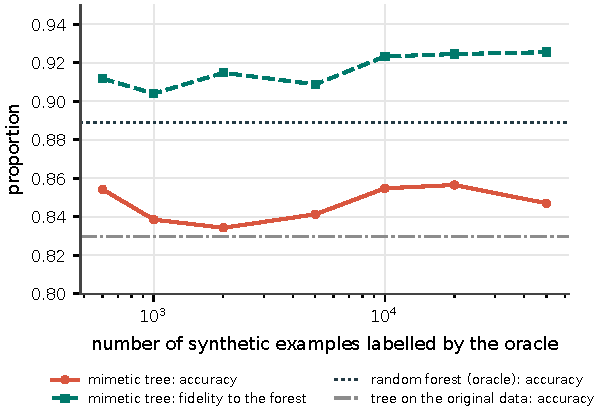
\includegraphics[width=0.74\textwidth]{ch02/mimetic}
\caption{Accuracy and fidelity of a 32-leaf mimetic tree as a function of the number of
synthetic examples labelled by a random forest, compared with the forest and with a 32-leaf tree
learned from the 600 original examples.}
\label{fig:mimetic}
\end{figure}

The same idea has been rediscovered several times. TREPAN \citep{craven1996extracting} extracted
trees from neural networks; \emph{model compression} \citep{bucila2006model} trained small neural
networks to imitate large ensembles; and \emph{knowledge distillation} \citep{hinton2015distilling}
trains a small network on the soft probabilities of a large one, and is today a standard way of
deploying large models, including language models, at a lower cost.

\subsection{Explanations, Clever Hans and security}

Imitating a model is also the basis of many \emph{explanation} methods, studied in Unit~3. LIME\index{LIME}
\citep{ribeiro2016should} explains the decision of any classifier $f$ on an example $x$ locally:
it samples perturbed examples around $x$, labels them with $f$, weights them by their proximity
to $x$ with a kernel $\pi_x$, and learns a simple (for example, sparse linear) model $g$ that
approximates $f$ well in the vicinity of $x$,
\begin{equation}
  \xi(x)=\argmin_{g\in G}\ \mathcal L(f,g,\pi_x)+\Omega(g),
\end{equation}
where $\Omega$ penalises the complexity of $g$. A mimetic\index{mimetic classifier} classifier is a \emph{global} surrogate\index{global surrogate};
LIME is a \emph{local} one.

Explanations matter because a model can be accurate for the wrong reasons. Clever Hans was a
horse that, at the beginning of the twentieth century, seemed able to do arithmetic; in fact it
was reading involuntary cues in the body language of its questioners. Ian Goodfellow compared
machine learning to Clever Hans: a model learns how to obtain its reward (for instance, a high
accuracy at labelling images), but not necessarily using the right cues. \citet{lapuschkin2019unmasking}
showed real examples: a classifier recognised horses in the PASCAL VOC images by detecting a
copyright tag present in many horse pictures, and added the label ``horse'' to a car when the tag
was pasted on its picture. In natural language processing, a model that seemed to reason about
arguments was found to exploit spurious lexical cues of the data set \citep{niven2019probing}.

This connects ensembles with security. We need to be sure that the model really learns the right
concept, which is difficult with black-box models. In software, using open-source libraries
allows anyone to inspect the code and to find and correct bugs; in machine learning this is not
always possible, since the behaviour of a model is in its parameters, not in its code. Using
comprehensible\index{comprehensibility} models where possible, studying the vulnerabilities of the most used frameworks,
and checking what models have learned are part of building reliable systems (Unit~3). Mimetic
models are also used by attackers: querying a deployed model and training a copy of it allows
its parameters to be stolen \citep{tramer2016stealing} and adversarial examples\index{adversarial example} that fool the
original to be crafted \citep{papernot2017practical}.

% ---------------------------------------------------------------------
\section{Ensembles in practice}\label{sec:enspractice}

\Cref{tab:enshyper} summarises the hyperparameters that matter most for the ensembles of this
unit. Some general recommendations:
\begin{itemize}
  \item start with a random forest (robust, few hyperparameters, OOB\index{out-of-bag estimate} estimate for free) and a
        gradient boosting\index{gradient boosting} model with early stopping\index{early stopping}; on tabular data one of them is usually
        hard to beat;
  \item tune with nested or held-out validation (\cref{sec:protocols}), never on the test data;
        and remember that, with many candidates, small differences are likely to be noise
        (\cref{sec:stats});
  \item boosted models and the averaged probabilities of forests are often miscalibrated:
        calibrate them if probabilities matter (\cref{sec:calibration});
  \item impurity-based\index{feature importance} feature importances of tree ensembles are biased towards attributes with
        many values; prefer permutation importance\index{feature importance!permutation} on held-out data \citep{strobl2007bias};
  \item if comprehensibility\index{comprehensibility}, latency\index{latency} or test costs\index{test costs} matter, consider pruning, delegation\index{delegation} or
        mimetic\index{mimetic classifier} models before deploying a large ensemble.
\end{itemize}

\begin{table}[htbp]
\centering\small
\caption{Hyperparameters that matter most in common ensembles (scikit-learn names).}\label{tab:enshyper}
\begin{tabularx}{\textwidth}{@{}>{\raggedright\arraybackslash}p{3.0cm}>{\raggedright\arraybackslash}X@{}}
\toprule
Method & Main hyperparameters and advice\\
\midrule
Bagging & \code{n_estimators} (more members usually stabilise the results, with diminishing returns); unstable base models (deep trees)\\
Random forest & \code{max_features} ($\sqrt M$ for classification); \code{n_estimators} (a few hundred);
\code{min_samples_leaf} to smooth probabilities; \code{oob_score=True} for a free estimate\\
Extra trees & as random forests; often slightly better and faster, sometimes needs more trees\\
AdaBoost & base learner depth (stumps or small trees); \code{n_estimators} and \code{learning_rate}
jointly; avoid with noisy labels\\
Gradient boosting & \code{learning_rate} (0.01--0.1) with early stopping; tree size
(\code{max_depth} or \code{max_leaf_nodes}); subsampling and regularisation\\
Stacking & diverse, reasonably good base models; simple metamodel; cross-validated meta-features\\
\bottomrule
\end{tabularx}
\end{table}

% ---------------------------------------------------------------------
\section{Summary}\label{sec:summary2}

\begin{itemize}
  \item Ensemble learning provides different methods that can improve the predictions of models.
        Combinations work when their members are both good (better than random) and diverse:
        Condorcet\index{Condorcet's jury theorem}'s theorem and the ambiguity decomposition\index{ambiguity decomposition} make this precise.
  \item Diversity\index{diversity} can be generated by manipulating the training examples, the features, the
        classes or the learning process, implicitly or explicitly, and can be measured with
        pairwise statistics and kappa--error\index{kappa--error diagram} diagrams.
  \item Predictions can be fused by averaging, multiplying, voting\index{voting}, Bayesian model averaging\index{Bayesian model averaging} or a
        learned metamodel; uniform averaging is simple and hard to beat.
  \item Bagging\index{bagging} and random forests reduce variance and degrade gracefully with label noise\index{label noise}; boosting
        reduces bias and is often more accurate on clean data, but AdaBoost\index{AdaBoost}, with its exponential loss,
        is sensitive to label noise (for gradient boosting\index{gradient boosting} it depends on the loss). Experimental
        comparisons show that random forests and boosted trees remain strong baselines on tabular data.
  \item Hybrid models (voting, stacking\index{stacking}, cascading\index{cascading}, mixtures of experts\index{mixture of experts}) combine different
        techniques and usually improve performance, provided the combination is learned on fresh
        data.
  \item A model can also know when not to predict. Abstaining is optimal when every prediction
        costs more than abstaining; for two classes, the window rule\index{window rule} of cautious classifiers\index{cautious classifier} with a
        cost-matched class bias is exactly the optimal reject rule. Cautious classifiers are
        evaluated by their accuracy--abstention\index{abstention} trade-off, which depends on how well their
        confidence ranks their own mistakes. Delegating\index{delegation} classifiers pass uncertain cases to a
        specialist, to a stronger but costlier model (a cascade) or to a person.
  \item The main drawbacks of combinations are comprehensibility\index{comprehensibility}, resources, test costs\index{test costs} and slower
        predictions; pruning, delegation and mimetic\index{mimetic classifier} models (distillation\index{model distillation}) mitigate them.
\end{itemize}

\section*{Bibliographic notes}
\phantomsection\addcontentsline{toc}{section}{Bibliographic notes}

\citet{kuncheva2014combining} is the reference textbook on combining classifiers, and
\citet{zhou2012ensemble} gives a concise and modern treatment of ensemble methods with their theory;
\citet{kyriakides2019hands} is a practical introduction in Python. \citet{dietterich2000ensemble}
remains an excellent short overview of why ensembles work, and \citet{brown2005diversity} survey the
methods for creating diversity\index{diversity}. Chapters~8, 10, 15 and~16 of \citet{hastie2009elements} cover
bagging\index{bagging}, boosting, random forests and ensemble learning from the statistical point of view. The
original papers on bagging \citep{breiman1996bagging}, boosting \citep{freund1997decision}, random
forests \citep{breiman2001random}, stacking\index{stacking} \citep{wolpert1992stacked}, cascade generalisation\index{cascading}\index{generalisation}
\citep{gama2000cascade} and mixtures of experts\index{mixture of experts} \citep{jacobs1991adaptive} are all very readable.
Cautious\index{cautious classifier} and delegating\index{delegation} classifiers are introduced in \citet{ferri2004cautious} and
\citet{ferri2004delegating}, and \citet{hendrickx2024machine} survey learning with a reject option\index{abstention};
\citet{mozannar2020consistent} and \citet{chen2023frugalgpt} are good entry points to learning to defer
and to model cascades.

\section*{Exercises}
\phantomsection\addcontentsline{toc}{section}{Exercises}

\begin{enumerate}[label=\textbf{2.\arabic*},ref=2.\arabic*,leftmargin=*,itemsep=6pt]
  \item\label{exr2:condorcet} Three independent classifiers are each right with probability 0.7.
        What is the probability that their majority vote\index{voting} is right? And for five classifiers?
  \item\label{exr2:fusion} Three models assign the probabilities $(0.70,0.25,0.05)$,
        $(0.10,0.50,0.40)$ and $(0.45,0.40,0.15)$ to the classes $(a,b,c)$. Which class is predicted
        by majority voting, by the linear combiner\index{linear combiner} and by the product combiner\index{product combiner}? Explain the
        difference.
  \item\label{exr2:bootstrap} What is the probability that a given example appears at least once
        in a bootstrap\index{bootstrap} sample of a data set with $n=10$ examples? And when $n\to\infty$?
  \item\label{exr2:variance} The members of a bagged ensemble have predictions with variance 1 and
        pairwise correlation 0.4. Compute the variance of the average of 10 members and of
        infinitely many members. What does a random forest try to change?
  \item\label{exr2:ada} In the first round of AdaBoost\index{AdaBoost} on 10 examples with uniform weights, the
        model misclassifies two examples. Compute $\varepsilon_1$, $\alpha_1$ and the new weights.
  \item\label{exr2:ambiguity} Two regression models predict 3 and 5 for an example whose target is
        4.5. Compute the ensemble error, the average error and the ambiguity\index{ambiguity decomposition}, and check
        \cref{eq:ambiguity}.
  \item\label{exr2:cautious} A cautious\index{cautious classifier} binary classifier gives the following matrix on 200 examples
        (rows: predicted $+$, $-$, $\perp$; columns: actual $+$, $-$): $(70,5)$, $(8,90)$,
        $(12,15)$. Compute coverage\index{coverage}, abstention\index{abstention}, accuracy and error, and check the relation between
        them.
  \item\label{exr2:rule} Apply the decision rule\index{decision rules} of \cref{sec:cautious} with $K=(0.6,0.4)$ and
        $w=0.5$ to the probability vectors $(0.9,0.1)$, $(0.7,0.3)$, $(0.55,0.45)$ and $(0.2,0.8)$.
  \item\label{exr2:chow} Abstaining costs 0.2 and an error costs 1. Should a calibrated classifier
        that predicts $(0.75,0.25)$ abstain? From which maximum probability is predicting better?
  \item\label{exr2:costcautious} With the cost matrix\index{cost matrix} of \cref{ex:costcautious}, what is the best
        decision for an example with probabilities $(0.2,0.3,0.5)$?
  \item\label{exr2:delegation} In a two-step delegation\index{delegation}, the first classifier keeps 70\% of the
        test examples with an accuracy of 0.95, and the second classifies the remaining 30\% with an
        accuracy of 0.75. What is the overall accuracy?
  \item\label{exr2:rebound} Continue Exercise~\ref{exr2:delegation}. The second classifier is
        confident on two thirds of the delegated examples (20\% of the total), where its accuracy
        is 0.85; on the remaining 10\% its accuracy is 0.55, whereas the first classifier would be
        right on 65\% of them. Check that the accuracy of the second classifier on all the
        delegated examples is 0.75, and compute the overall accuracy with and without round
        rebound\index{round rebound}. When does round rebound help?
  \item\label{exr2:window} False positives cost 1, false negatives cost 3 and abstaining costs
        0.4. Compute the optimal abstention band, the cost threshold $t^\star$ and the window
        $w^\star$ that makes the window rule\index{window rule} optimal, and check that the window rule abstains on
        the same band.
  \item\label{exr2:stacking} Explain why the metamodel of stacking\index{stacking} must be trained on out-of-fold
        predictions. What would happen if one of the base models were a 1-nearest neighbour\index{k-nearest neighbours@$k$-nearest neighbours}
        classifier and the metamodel were trained on its predictions on the training data?
  \item\label{exr2:mimetic} When can a mimetic\index{mimetic classifier} tree with lower accuracy than the ensemble still be
        preferable? Which quantity would you report besides its accuracy?
  \item\label{exr2:design} A fraud detection system must answer in less than 5 milliseconds, but the
        best model is a stacking of three large ensembles. Propose three ways of deploying something
        close to it within the time budget.
\end{enumerate}

\section*{Solutions to selected exercises}
\phantomsection\addcontentsline{toc}{section}{Solutions to selected exercises}

\begin{description}[font=\bfseries,leftmargin=0pt,itemsep=5pt]
  \item[\ref{exr2:condorcet}] $0.7^3+3\cdot0.7^2\cdot0.3=0.343+0.441=0.784$. For five classifiers,
        $10\cdot0.7^3\cdot0.3^2+5\cdot0.7^4\cdot0.3+0.7^5=0.309+0.360+0.168=0.837$.
  \item[\ref{exr2:fusion}] Votes: $a$, $b$, $a$, so voting\index{voting} predicts $a$. Average:
        $(0.417,0.383,0.200)$, so $a$. Normalised product: the products are $0.0315$, $0.050$ and
        $0.003$, so $b$: the low probability that the second model gives to $a$ acts as a veto.
  \item[\ref{exr2:bootstrap}] $1-(1-1/10)^{10}=1-0.349=0.651$; when $n\to\infty$, $1-e^{-1}=0.632$.
  \item[\ref{exr2:variance}] By \cref{eq:avgvar}, $0.4+0.6/10=0.46$ for 10 members and $0.4$ for
        infinitely many. A random forest decorrelates the trees to reduce $\rho$, the term that does
        not vanish.
  \item[\ref{exr2:ada}] $\varepsilon_1=0.2$, $\alpha_1=\frac12\ln4=0.693$. Before normalising, the two
        mistakes weigh $0.1\cdot2=0.2$ and the eight correct examples $0.1\cdot0.5=0.05$; after
        normalising (total 0.8), $0.25$ and $0.0625$: the mistakes carry half of the weight.
  \item[\ref{exr2:ambiguity}] $\bar f=4$, $E=0.25$; $\bar E=(2.25+0.25)/2=1.25$;
        $\bar A=(1+1)/2=1$; and $1.25-1=0.25$.
  \item[\ref{exr2:cautious}] $\mathit{Card}=200$, 173 classified: coverage\index{coverage} $0.865$, abstention\index{abstention}
        $0.135$; accuracy $160/173=0.925$; error $13/200=0.065$. Indeed
        $0.925\cdot0.865=0.80=0.865-0.065$.
  \item[\ref{exr2:rule}] $\tau=(0.4\cdot0.5+0.6,\ 0.6\cdot0.5+0.4)=(0.8,0.7)$. $(0.9,0.1)$: class 1;
        $(0.7,0.3)$: unknown; $(0.55,0.45)$: unknown; $(0.2,0.8)$: class 2.
  \item[\ref{exr2:chow}] Abstain if $\max_ip_i<1-0.2=0.8$, so yes: predicting has expected cost\index{expected cost}
        0.25, more than 0.2. Predicting is better from a maximum probability of 0.8.
  \item[\ref{exr2:costcautious}] Expected costs: $a$: $-0.5+1.2+1.0=1.7$; $b$: $0.42-1.05=-0.63$;
        $c$: $0.24+0.39-2.0=-1.37$; $\perp$: 0. The best decision is $c$.
  \item[\ref{exr2:delegation}] $0.7\cdot0.95+0.3\cdot0.75=0.665+0.225=0.89$.
  \item[\ref{exr2:rebound}] On the delegated 30\%, the second classifier is right on
        $0.2\cdot0.85+0.1\cdot0.55=0.225$ of the total, that is, $0.225/0.3=0.75$. Without rebound the
        overall accuracy is $0.665+0.225=0.89$; with rebound, the last 10\% is classified by the
        first classifier and the accuracy is $0.665+0.2\cdot0.85+0.1\cdot0.65=0.90$. Round rebound\index{round rebound}
        helps exactly when the first classifier is more accurate than the second on the cases that
        bounce back.
  \item[\ref{exr2:window}] Band: $0.4/3=0.133<p<1-0.4=0.6$. Then $t^\star=1/4=0.25$ and
        $w^\star=1-0.4\cdot4/3=0.467$, and the window is $0.25\cdot(1-0.467)=0.133<p<0.25+0.75\cdot0.467=0.6$.
  \item[\ref{exr2:stacking}] On its own training data a 1-NN classifier is always right, so a
        metamodel trained on those predictions would learn to trust it blindly, although its
        predictions on new data are much worse. Out-of-fold predictions show the metamodel how each
        base model behaves on unseen examples.
  \item[\ref{exr2:mimetic}] When comprehensibility\index{comprehensibility}, auditability, latency or test costs\index{test costs} matter more
        than a small loss of accuracy. Report its \emph{fidelity\index{fidelity|textbf}} to the ensemble, and its size.
  \item[\ref{exr2:design}] For instance: distil\index{model distillation} the stacking\index{stacking} into a single small model (mimetic\index{mimetic classifier}
        model or distillation); prune the ensembles\index{ensemble pruning}; or use a delegating\index{delegation} cascade\index{cascading} in which a fast
        model answers the easy cases and only the uncertain ones (within the budget) go to the
        expensive model.
\end{description}

